\section{The steady state}

The way to steady state described in
here remarks on the resulting profiles.

\subsection{Parallel profiles}
Consider: Remove ln(n), vortD, nui
%
\begin{figure}[htb]
    \centering
    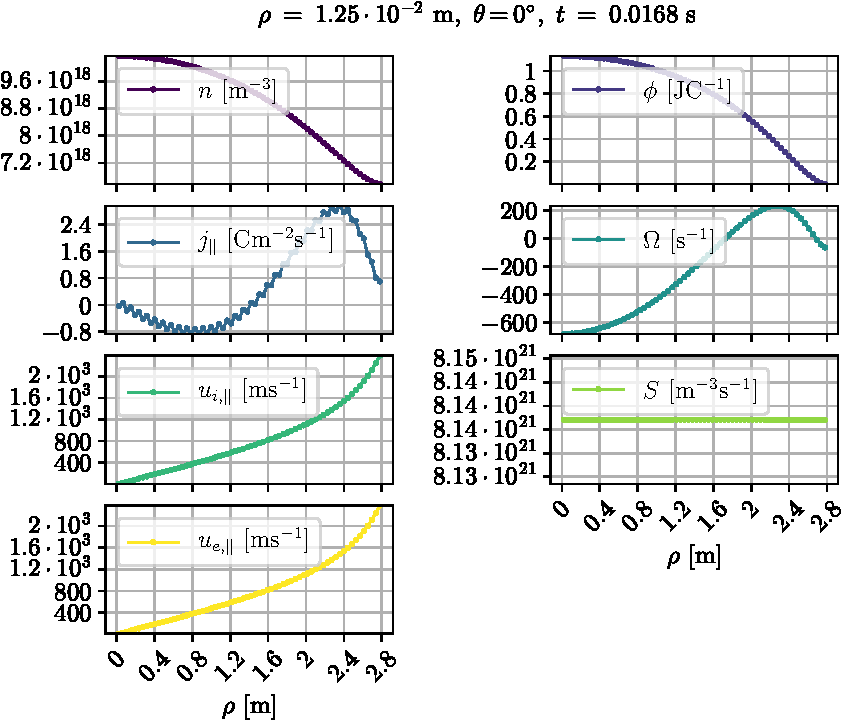
\includegraphics[width=1.0\textwidth]{fig/results/1DProfiles/B010Par}
    \caption{Parallel profiles in the steady state for $B=0.1\T$}
    \label{fig:parProfs}
\end{figure}


Parallel
The parallel profile is mainly determined by the source, the sheath condition and the boundary condition at the sheath entrance.
There exsists a threshold on the source for which below the threshold the plasma is completely emptied and no density profile is allowed to build up.
Above this threshold the parallel extent of the source determines the filling.
That is:
The parallel shape of the source has less to do with the shape of the parallel density profile than the parallel extent of the source.
If the boundary condition on the density was changed to for example the Cauchy boundary condition (described in ...)
the shape of the steady state profile would be much steeper close to the sheath entrance.
Such steep gradients may give rise to numerical instabilities if the spatial resolution is not increased.

We observe that the potential profile follows the density profile quite well.
This is expected as to the first order the pressure is balancing the electric field, as seen in the ordering described in....
and because we do not restric the potential by any parallel boundary condition.

Next, the parallel velocity profiles are mainly arising from the parallel boundary condition.
Both the ions and electrons are fixed to a zero velocity at the boundary opposite to the sheath.
The ions are further fixed to the ion sound velocity at the sheath entrance, whereas the electron velocity will regulate itself after the potential.
If more electrons than ions were to escape, a potential difference would build up attracting more ions and pushing away more electrons.

Why is it not ambipolar?

Any difference in the velocities would lead to currents.
The divergence of current must be constant as a consequence of charge conservation.
Any parallel derivatives in the parallel current not balancing the other terms in ...
would lead to an acceleration of the plasma spinnig.

Therefore, the perpendicular vorticity profile comes as a direct consequence of the parallel derivative of the current in that point.

\subsection{Perpendicular profiles}

\begin{figure}[htb]
    \centering
    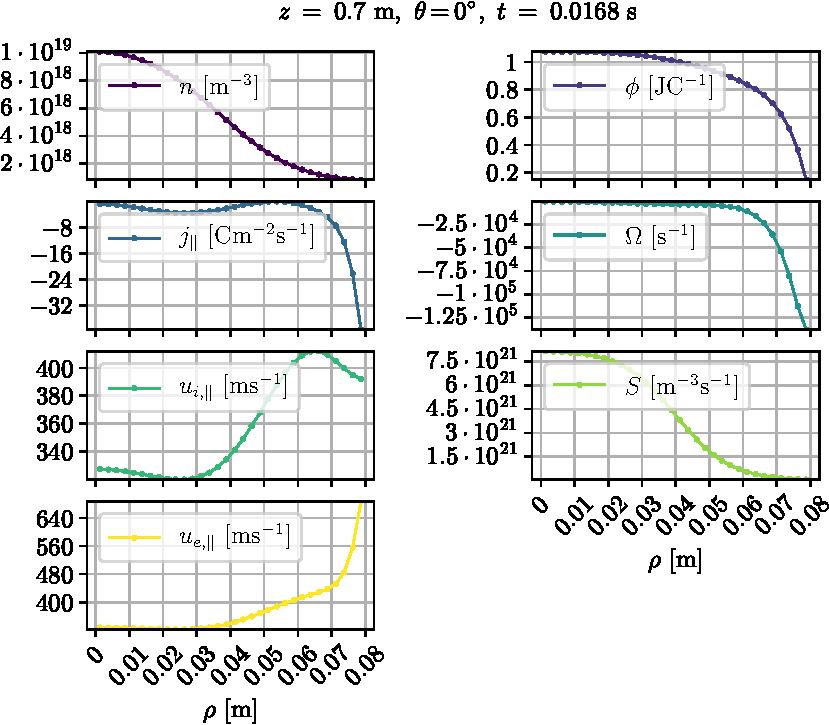
\includegraphics[width=1.0\textwidth]{fig/results/1DProfiles/B010Rad}
    \caption{Radial profiles in steady state for $B=0.1\T$}
    \label{fig:radProfs}
\end{figure}

Perpendicular profiles
As in the parallel direction, the shape of the perpendicular density profile is determined mainly by the source and the radial boundary conditions.
The radial extent of the source plays a larger role in determining the radial density profile than the shape of the source.

The perpendicular potential profile is a result of two effects.
Near the axis, the Boltzmann distribution follows induvidually for each radial position.
As we approach $L_\rho$ the radial potential profile will be effected by fixing the potential to $0$ at $L_\rho$.
This differs from the density profile because of the zero gradient enforcement on $n$ at $L_\rho$.

\section{The linear phase}
Linear phase, see growing and rotation.

Linear phase comes from unstabilities in linear set of equation.
No non-linearities are needed.
If only linear system, growth rates would continue forever.

Doesn't start by itself, but is seeded with a Gaussian noise with a level of on vortD
% FIXME; Could add arrow indicating direction of rotation
%
\begin{figure}[htbp]
    \centering
    \begin{subfigure}[h]{1.00\textwidth}
        \centering
        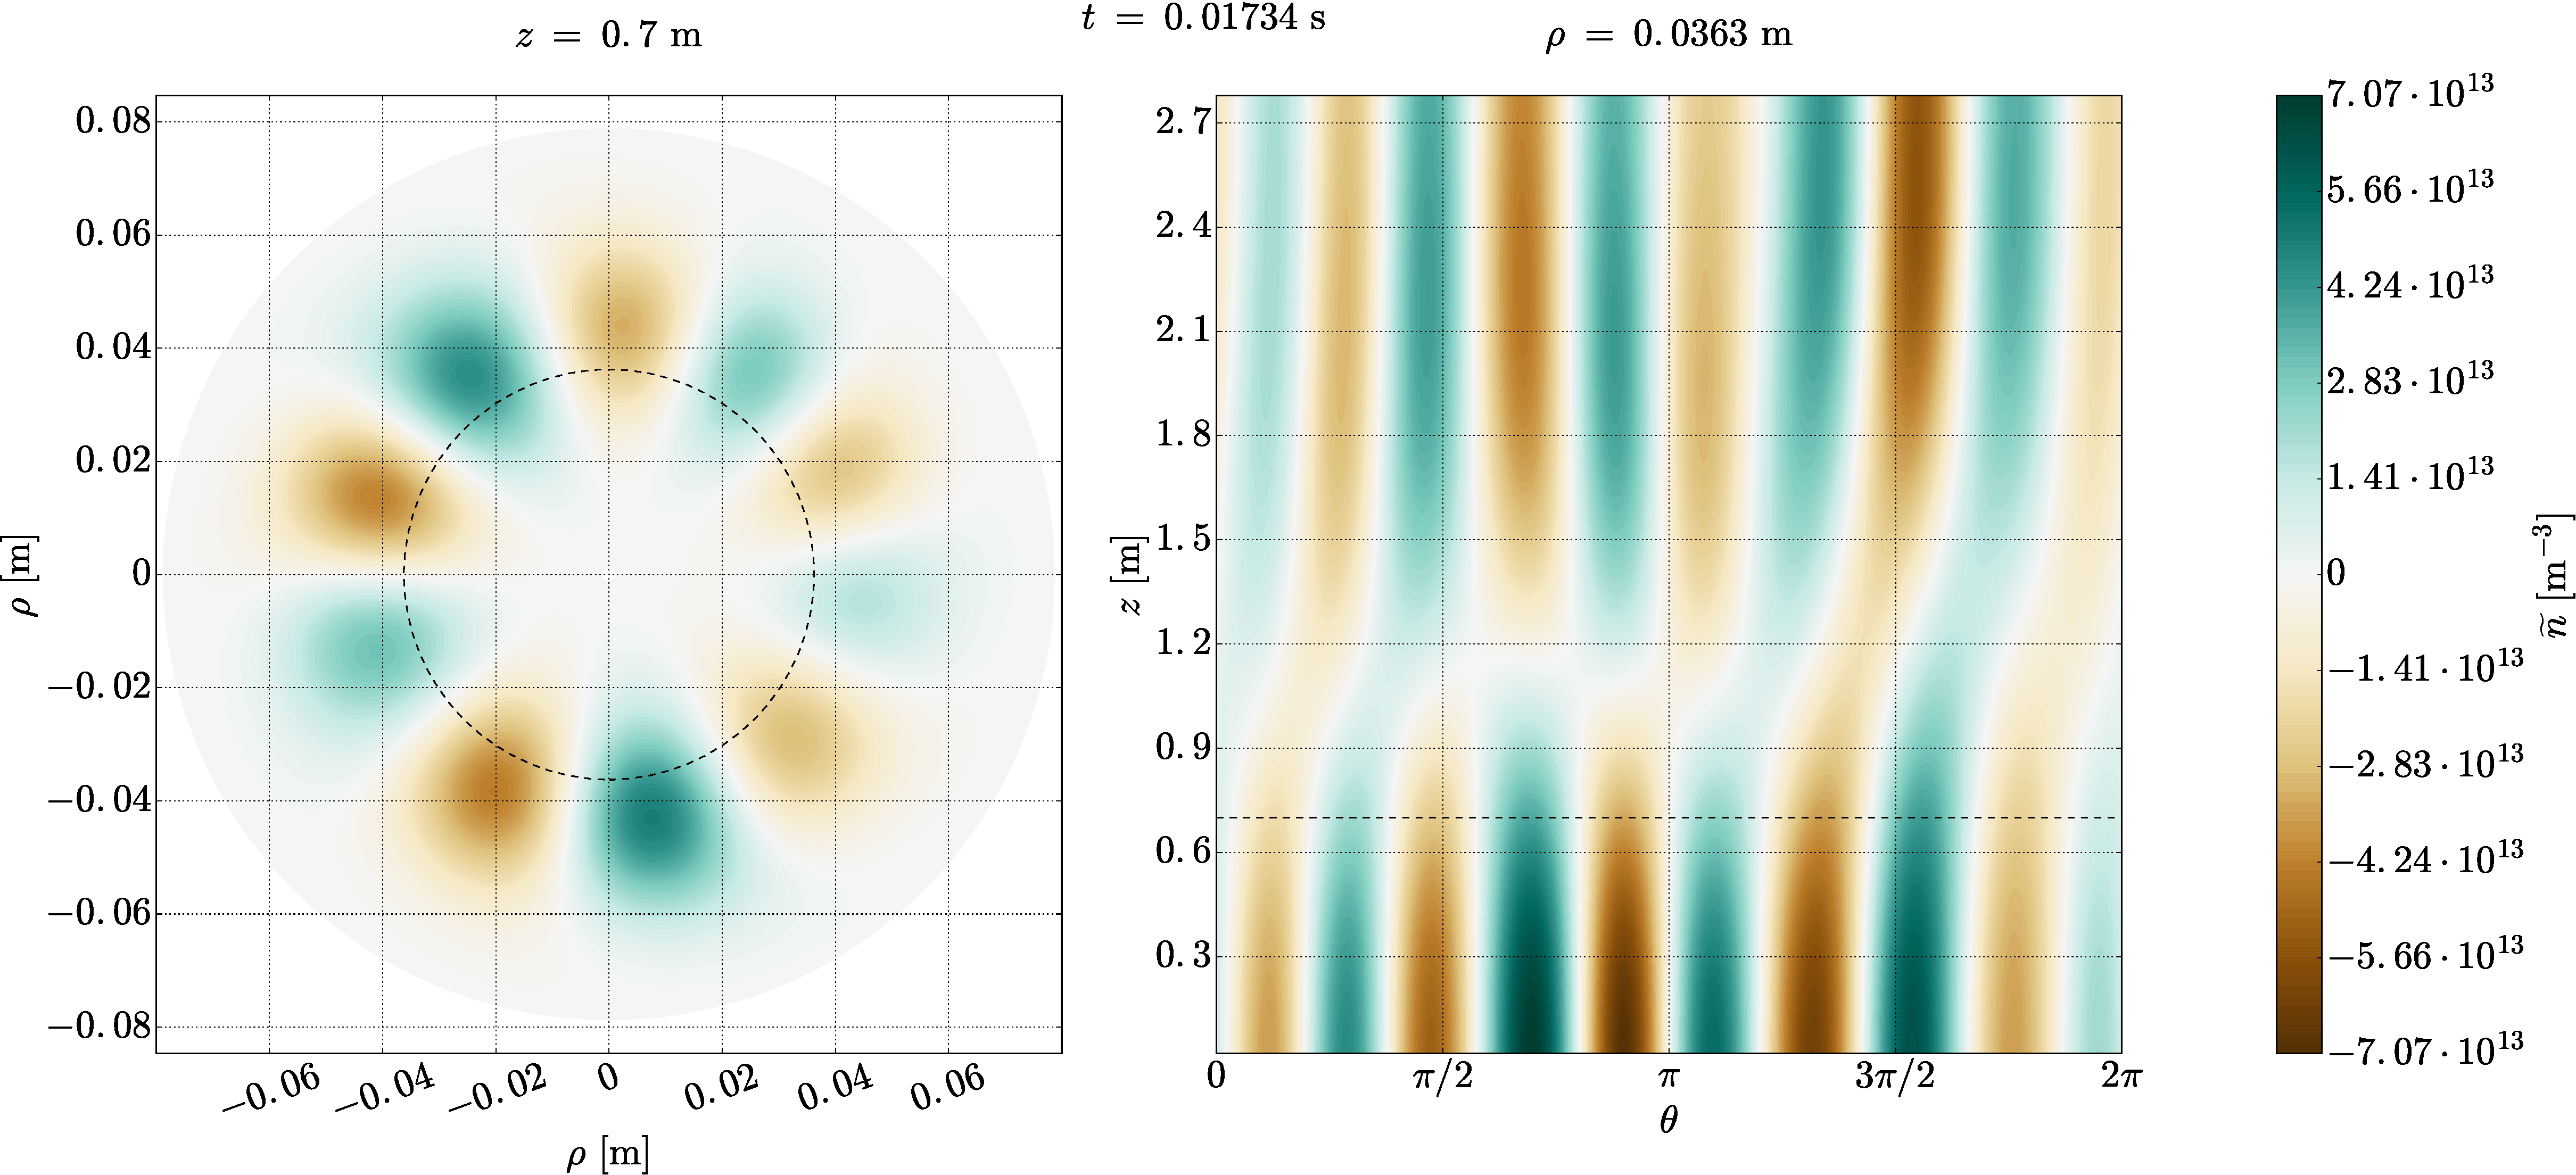
\includegraphics[width=1.0\textwidth]{fig/results/rotModes/n-perpPol-2D-fluct-0}
        \label{fig:rot1}
    \end{subfigure}%
    \\
    \begin{subfigure}[h]{1.00\textwidth}
        \centering
        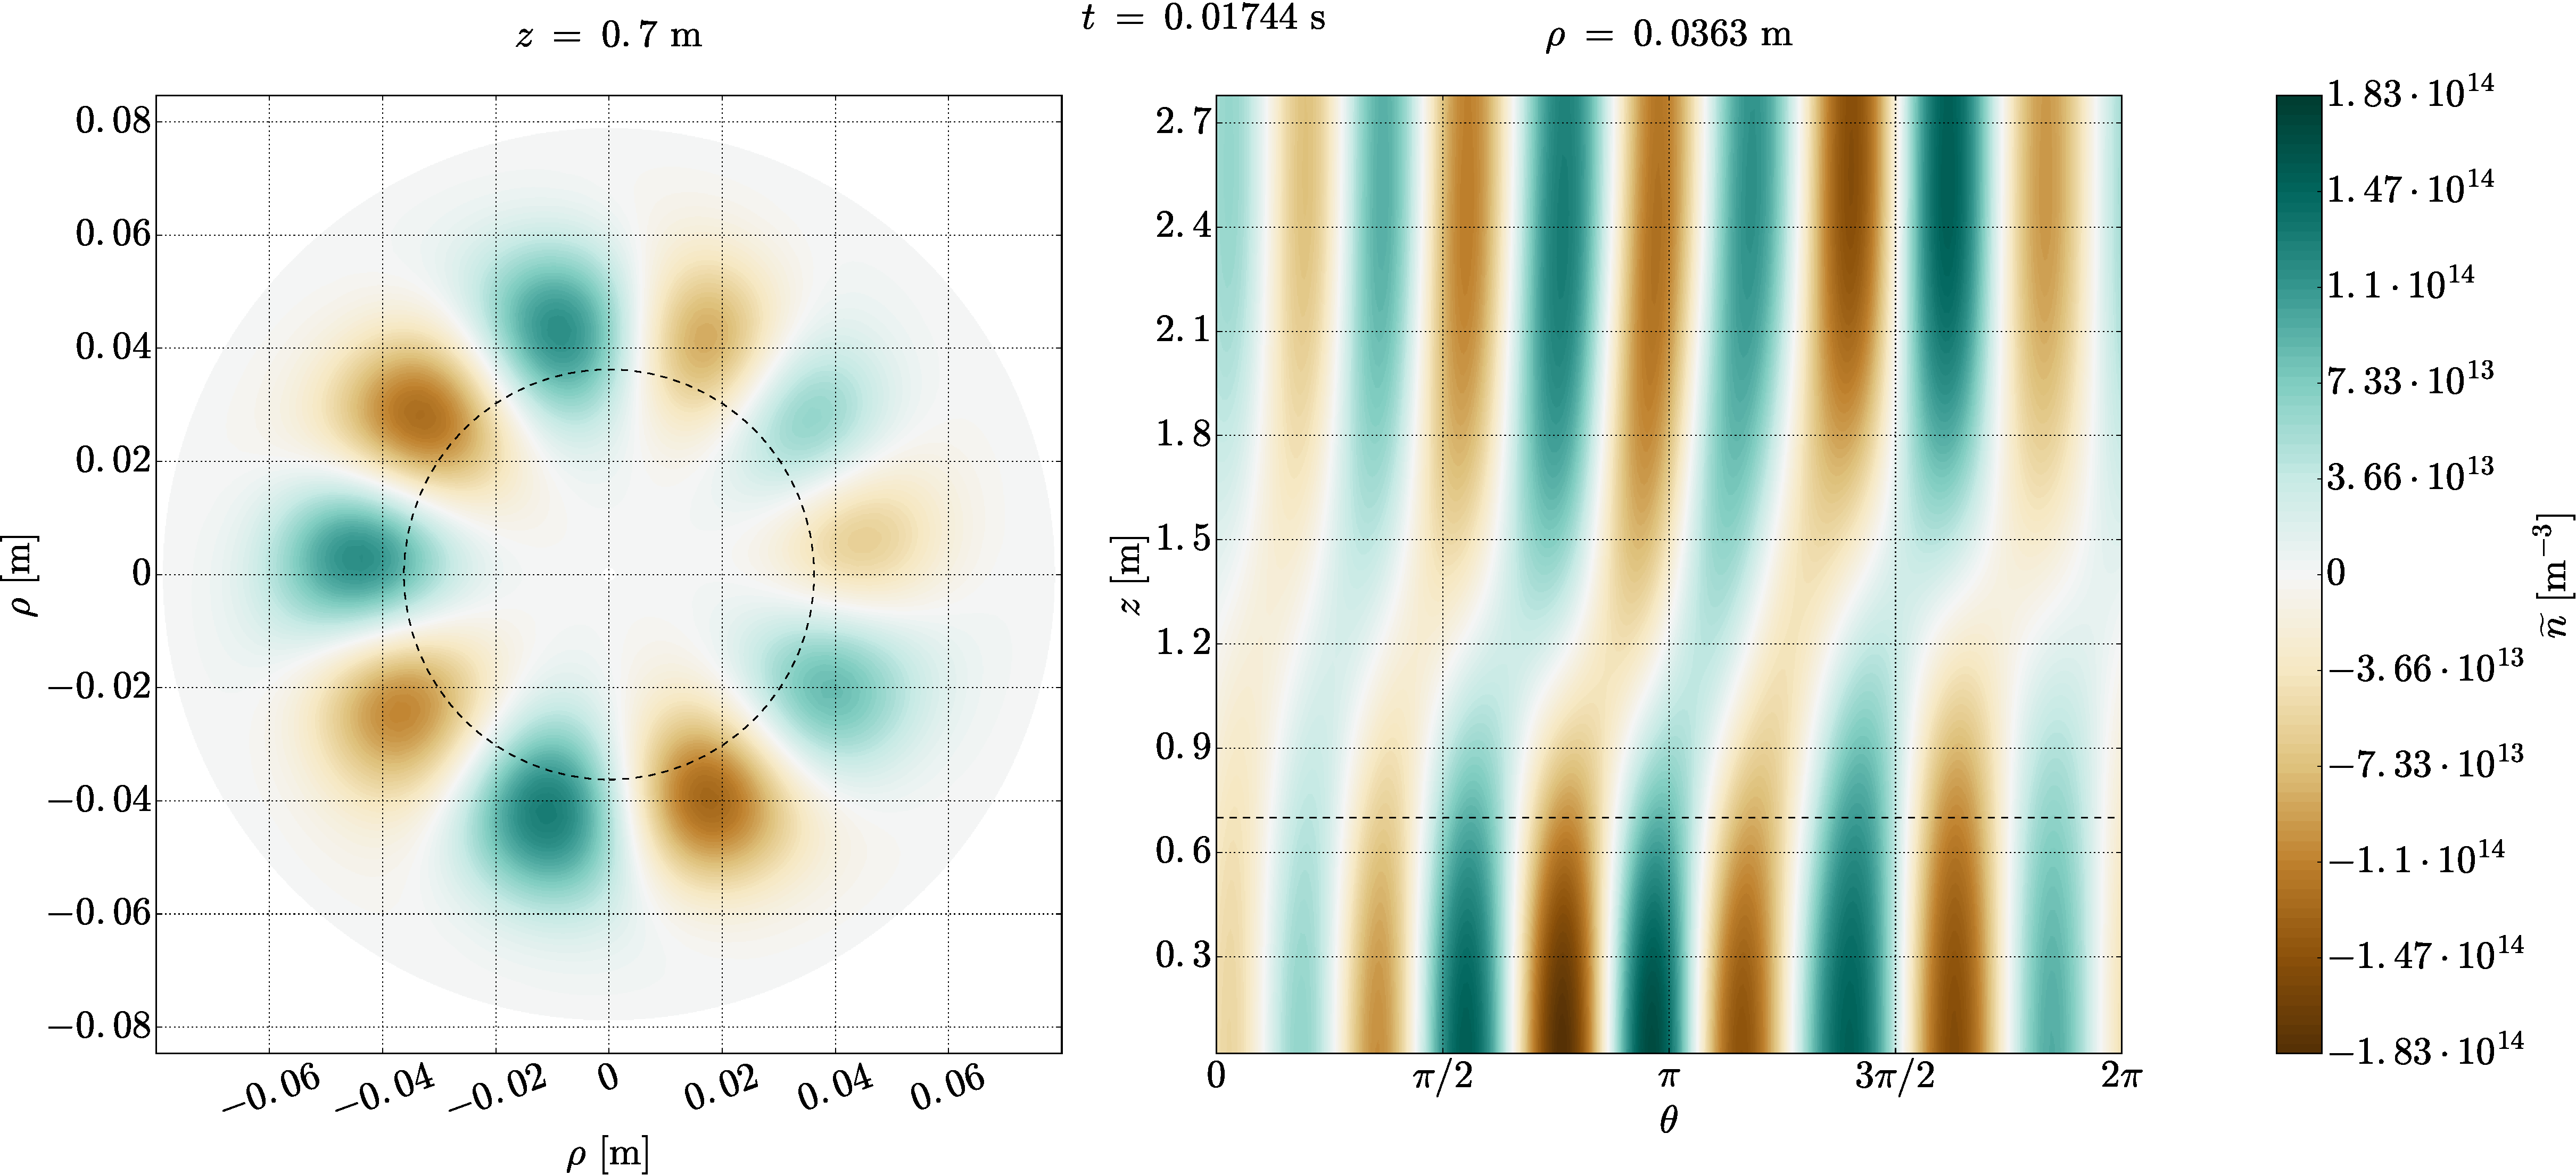
\includegraphics[width=1.0\textwidth]{fig/results/rotModes/n-perpPol-2D-fluct-1}
        \label{fig:rot2}
    \end{subfigure}
    \\
    \begin{subfigure}[h]{1.00\textwidth}
        \centering
        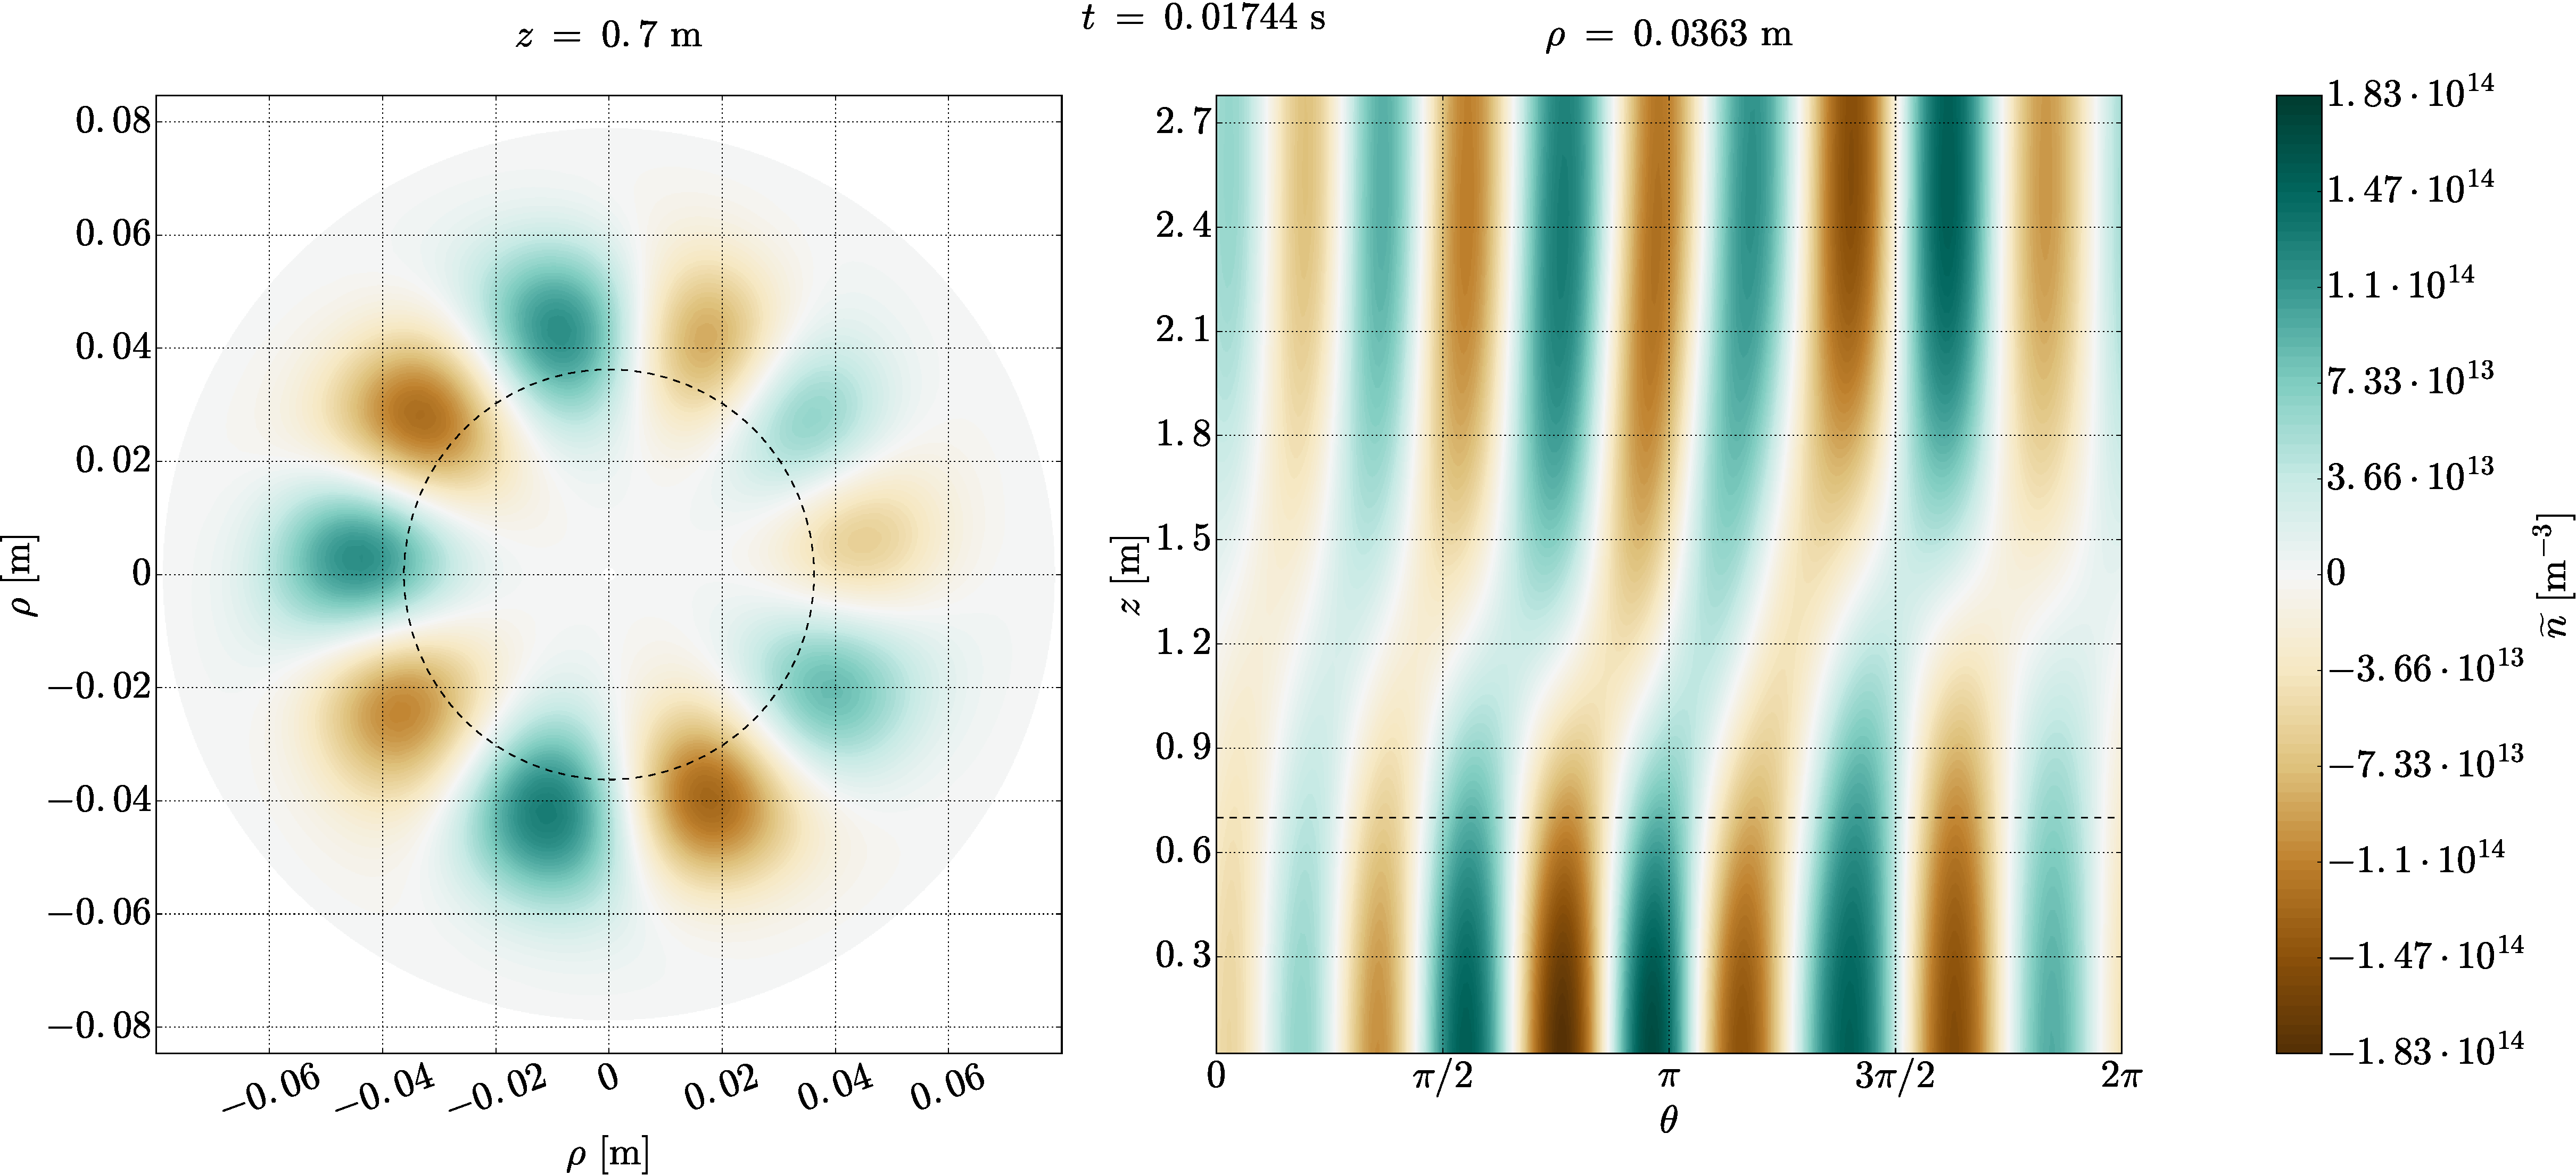
\includegraphics[width=1.0\textwidth]{fig/results/rotModes/n-perpPol-2D-fluct-2}
        \label{fig:rot3}
    \end{subfigure}
    \caption{Rotation of modes}
\end{figure}
%
Dominating mode is dependent on $B$, also, parallel mode moves
%
\begin{figure}[htbp]
    \centering
    \begin{subfigure}[h]{1.00\textwidth}
        \centering
        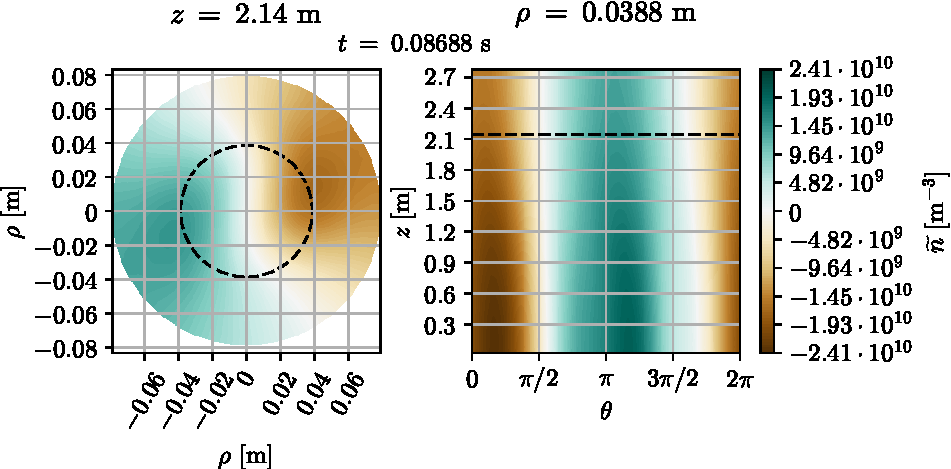
\includegraphics[width=1.0\textwidth]{fig/results/modesDiffScanVals/B002}
        \caption{$B=0.02 \T$}
        \label{fig:B002}
    \end{subfigure}%
    \\
    \begin{subfigure}[h]{1.00\textwidth}
        \centering
        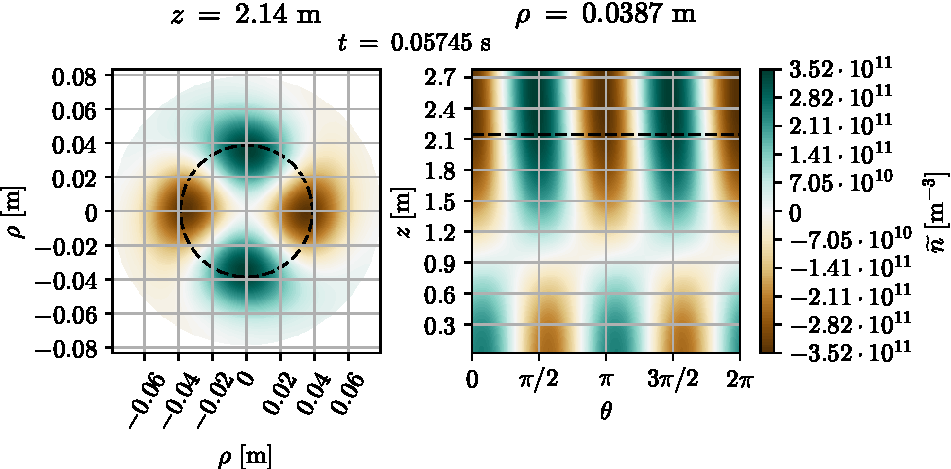
\includegraphics[width=1.0\textwidth]{fig/results/modesDiffScanVals/B004}
        \caption{$B=0.04 \T$}
        \label{fig:B004}
    \end{subfigure}
    \\
    \begin{subfigure}[h]{1.00\textwidth}
        \centering
        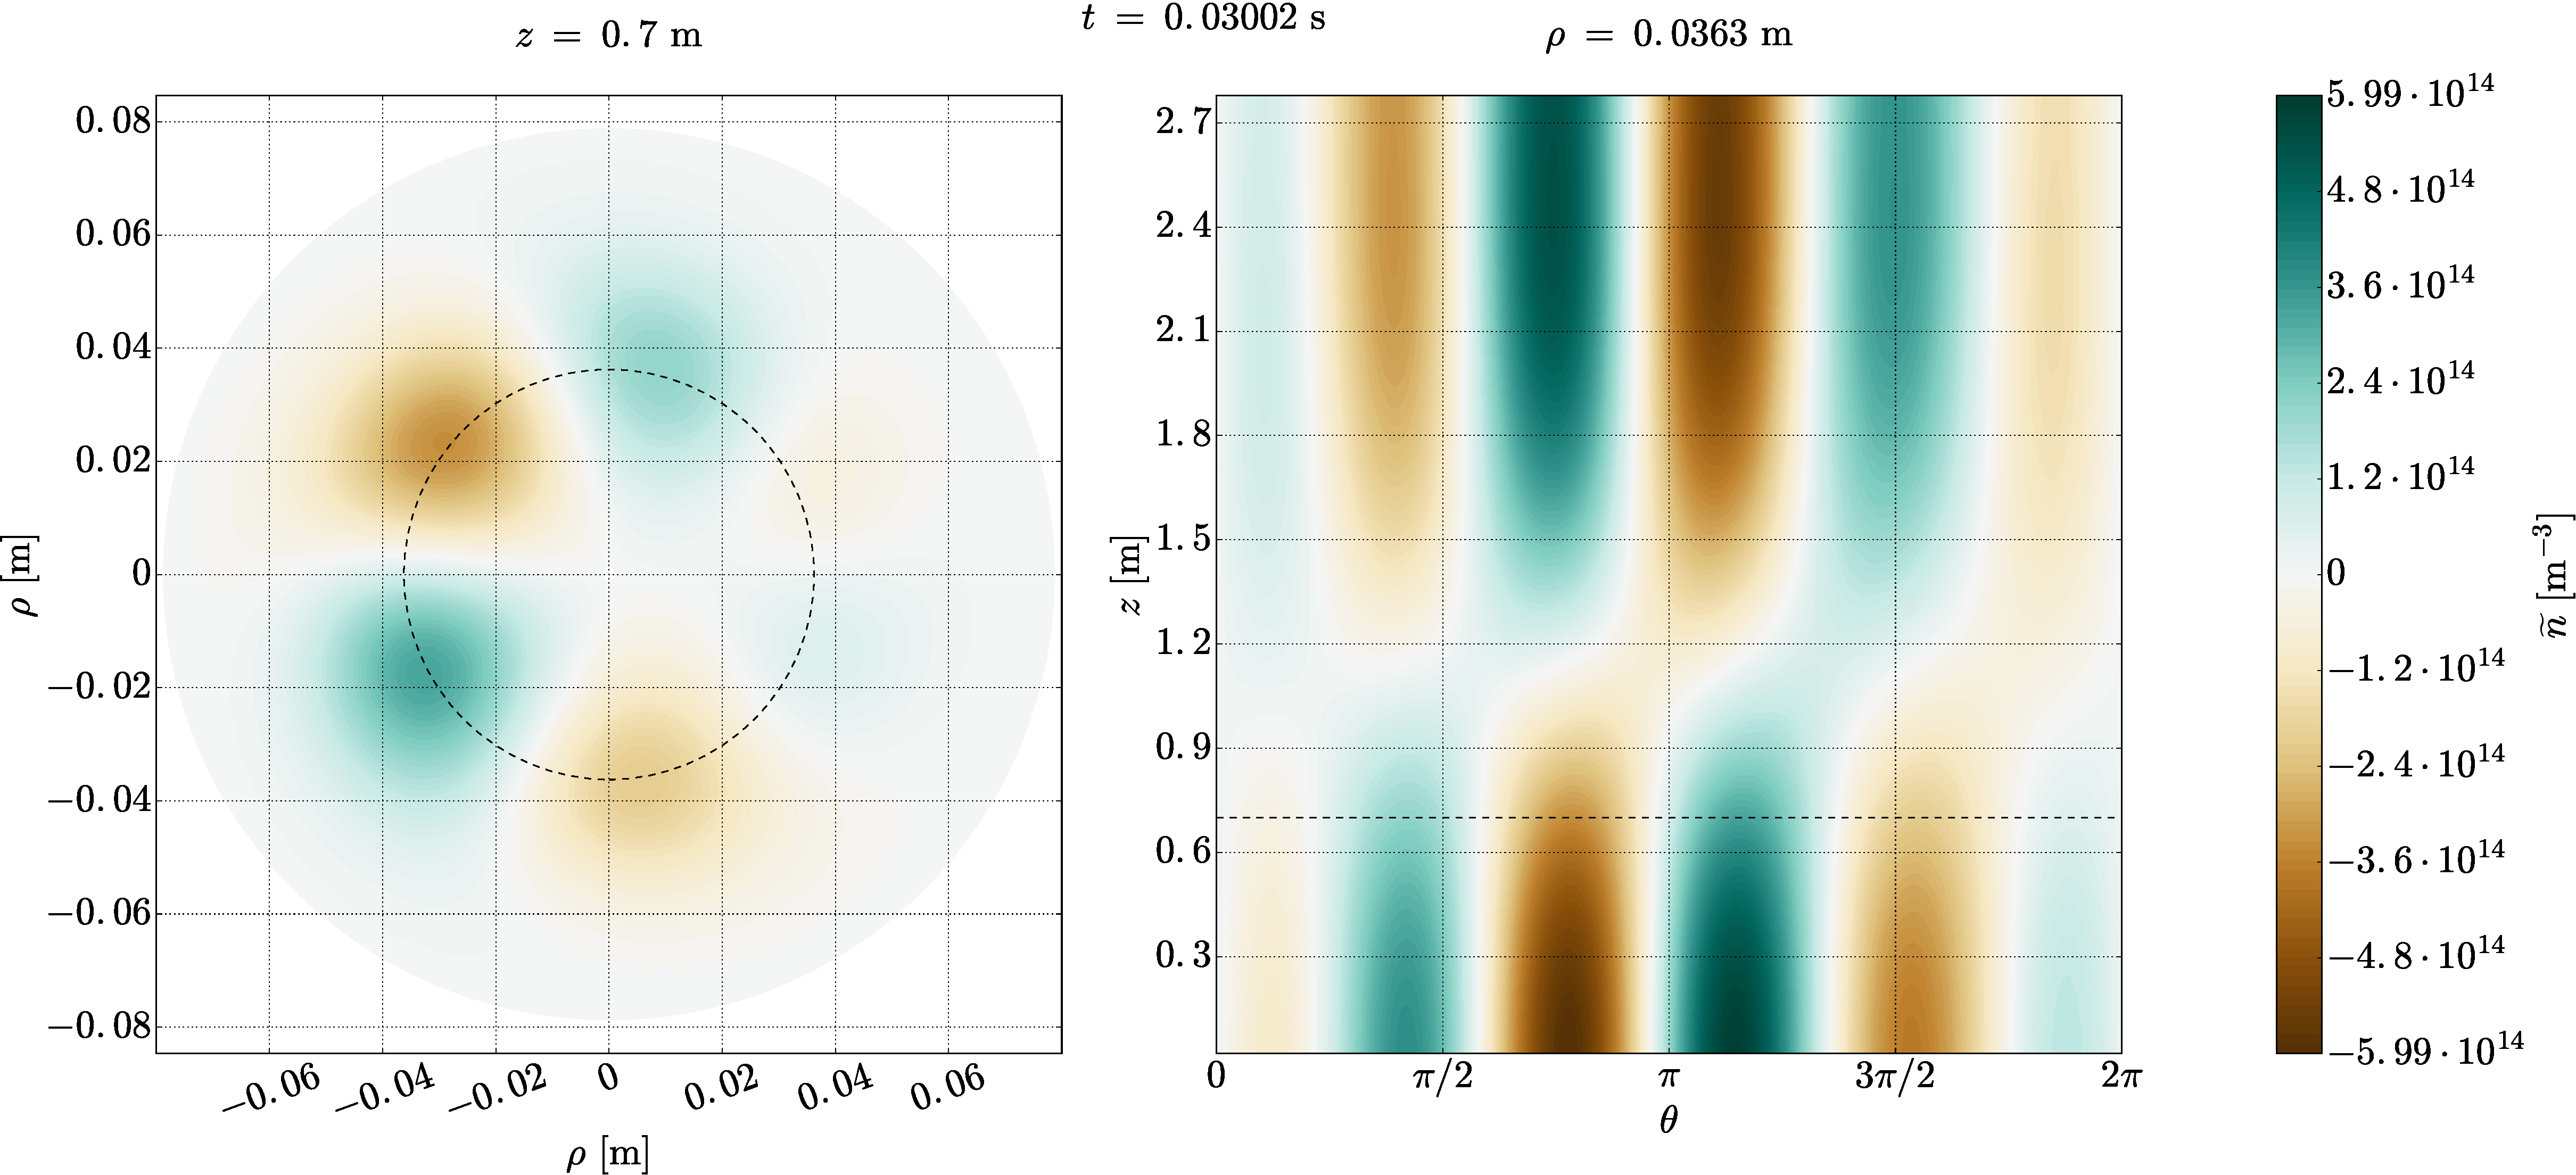
\includegraphics[width=1.0\textwidth]{fig/results/modesDiffScanVals/B006}
        \caption{$B=0.06 \T$}
        \label{fig:B006}
    \end{subfigure}
    \caption{Dominant mode depends on $B$}
\end{figure}
%
A more quantitative way to look at the linear phase is to plot the fourier modes at the position of the most unstable growth.
From theory, this coincides with the position of largest gradient.
As the abscissa is logarithmic, exponential grow will appear as straigth lines
%
\begin{figure}[htbp]
    \centering
    \begin{subfigure}[h]{1.00\textwidth}
        \centering
        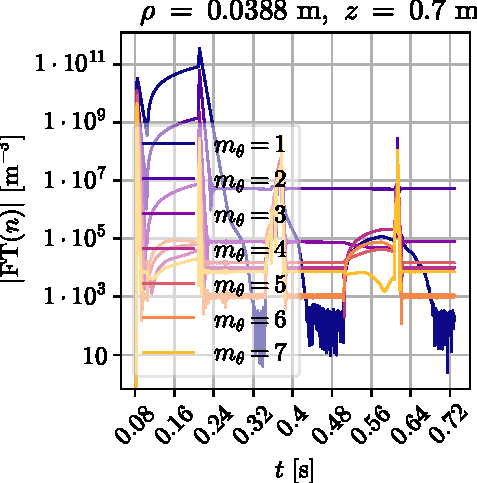
\includegraphics[width=1.0\textwidth]{fig/results/fourierModes/stable}
        \label{fig:fourierStable}
        \caption{For $B=0.02\T$ the system is stable against perturbation}
    \end{subfigure}%
    \\
    \begin{subfigure}[h]{1.00\textwidth}
        \centering
        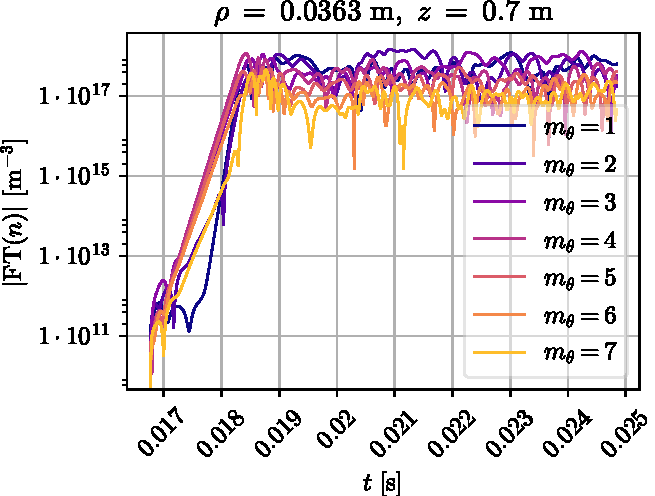
\includegraphics[width=1.0\textwidth]{fig/results/fourierModes/unstable}
        \label{fig:fourierUnstable}
        \caption{Growth rate leading to saturated turbulence for $B=0.1\T$}
    \end{subfigure}
    \caption{Time trace of the Fourier modes.}
\end{figure}
%
Can be summarized in growth rates plot
where the start and the end of the linear phase has been determined by visual inspection.
The start has been defined as the time where the initial perturbation has vanished, and where the modes start to show a more or less exponential growth.
The end is defined as the time where any mode, which up to that point in time has been flat or damped suddenly shows an exponential growth.



Assuming perturbation on the from $A\exp\L(i[k_\theta \theta - \L(i\Im[\om] + \Re[\om]\R) t]\R)$, where one can assure oneself that positive $\Im(\om)$ causes exponential growth, and a positive $\Re(\om)$ causes a counter-clockwise rotation of the perturbation if $\theta$ grows in the counter-clockwise direction, as the inverse wavelength $k_\theta$ stays constant.
%
\begin{figure}[htbp]
    \centering
    \begin{subfigure}[h]{1.00\textwidth}
        \centering
        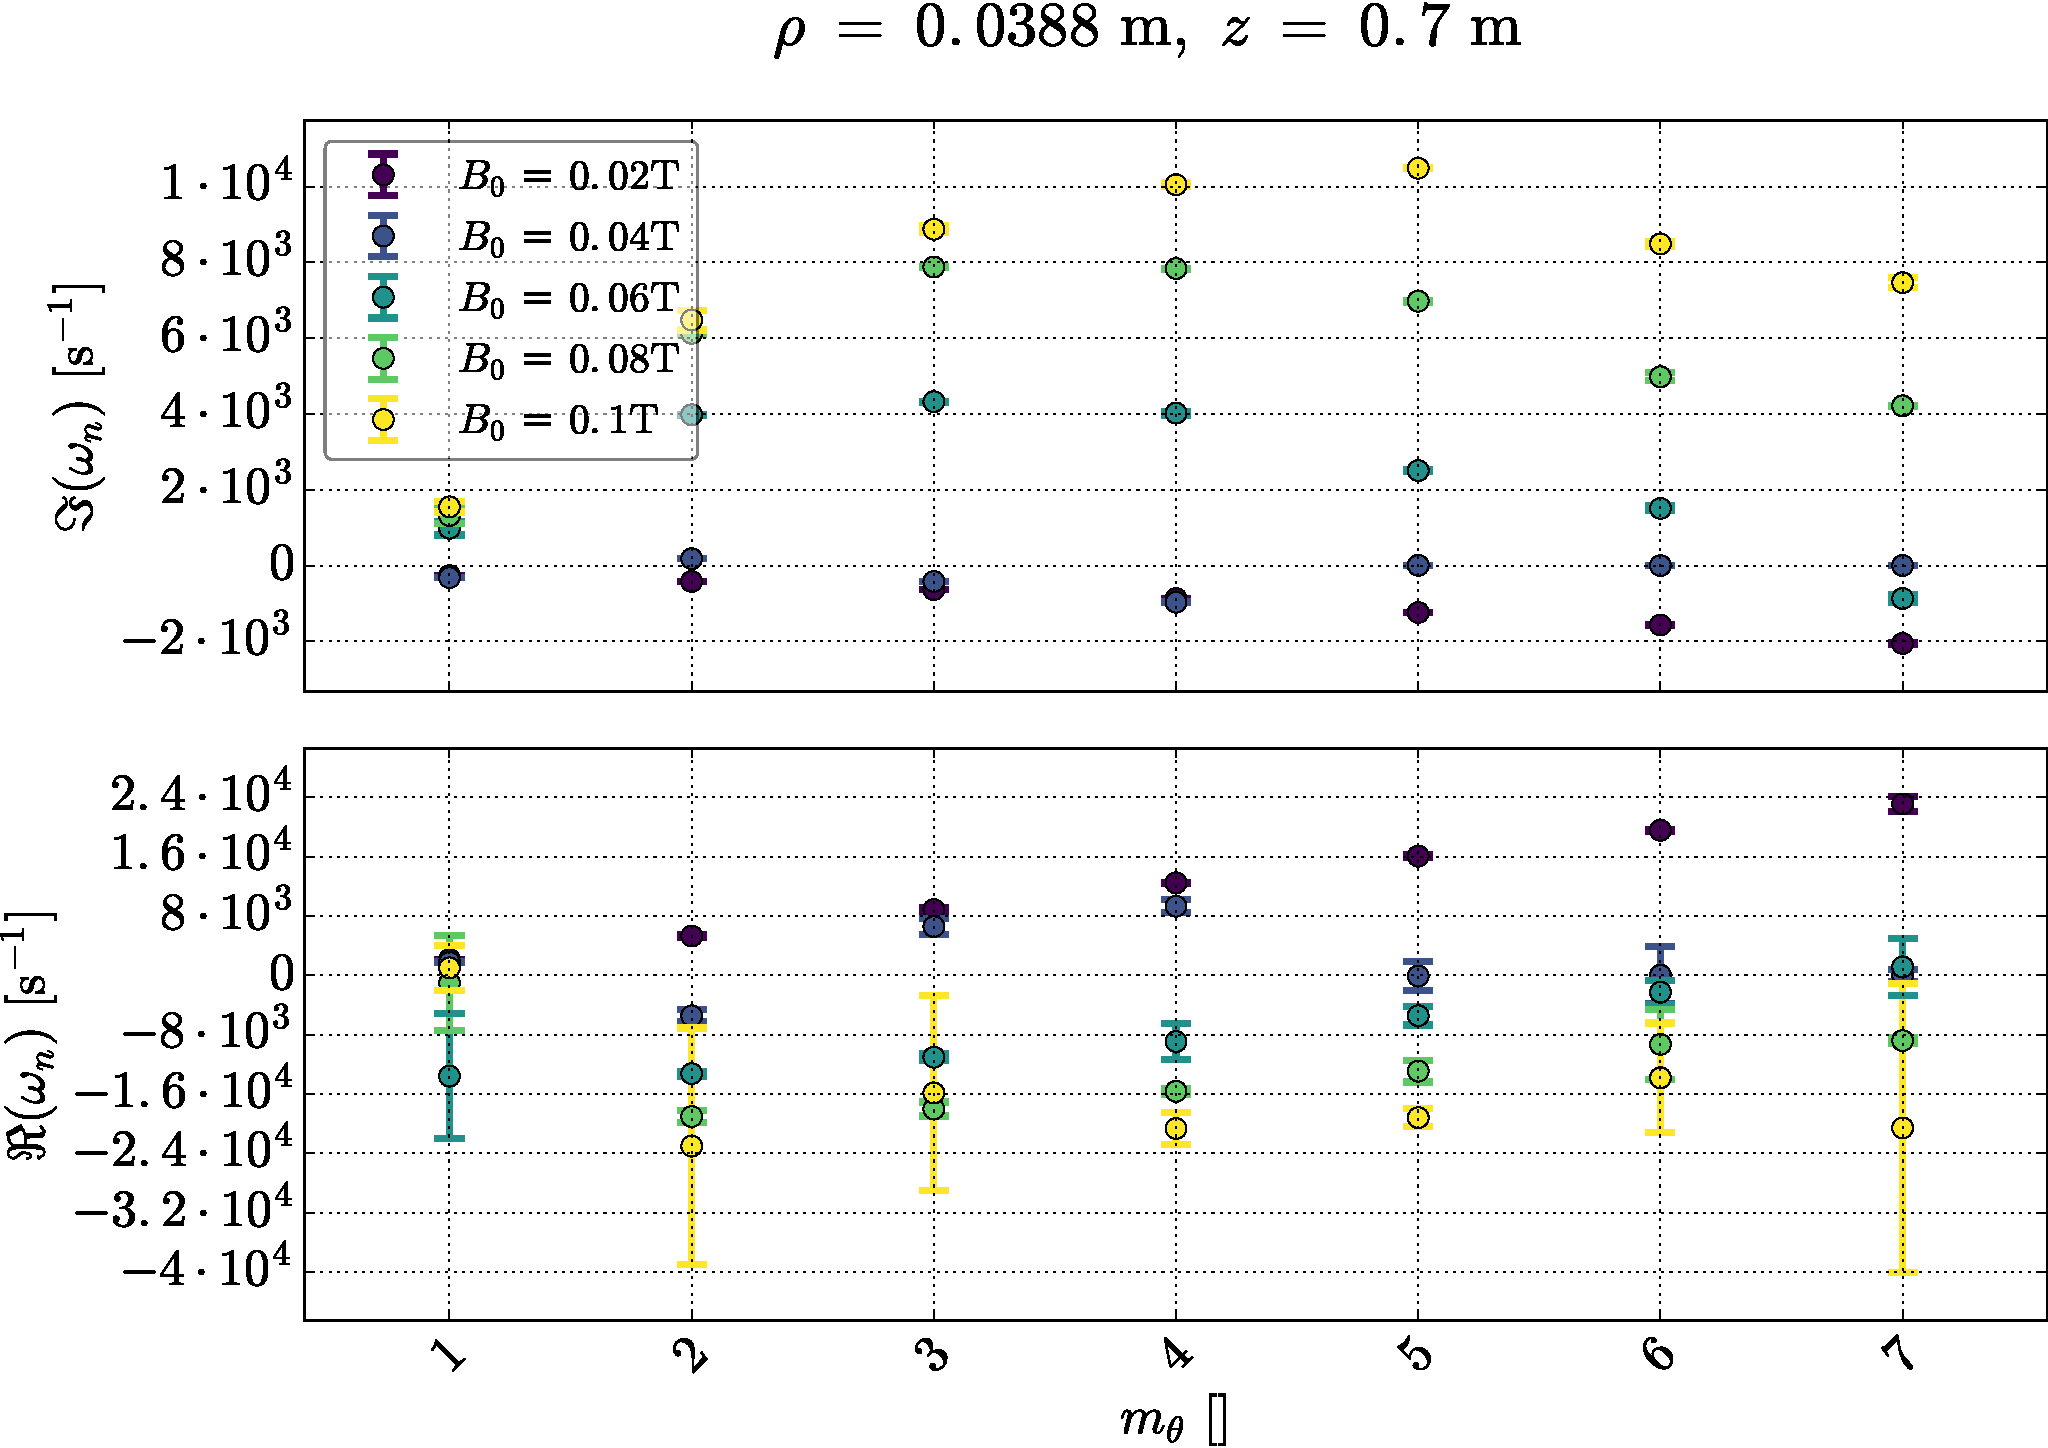
\includegraphics[width=1.0\textwidth]{fig/results/growthRates/growthRatesB0}
        \label{fig:grB}
    \end{subfigure}%
    \\
    \begin{subfigure}[h]{1.00\textwidth}
        \centering
        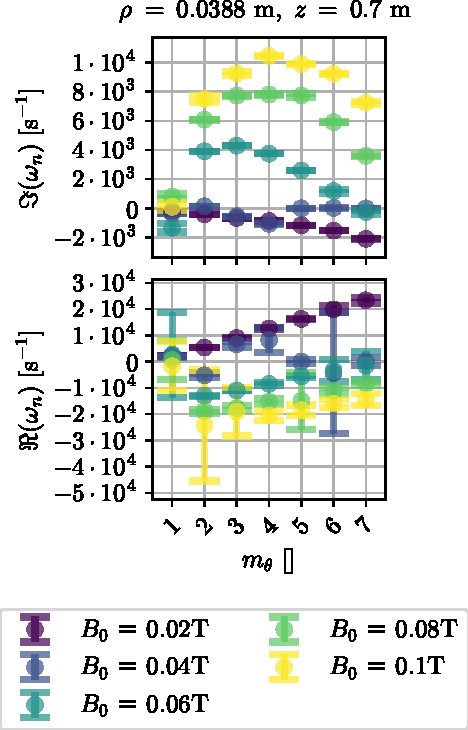
\includegraphics[width=1.0\textwidth]{fig/results/growthRates/growthRatesB0ModeNr}
        \label{fig:grBModeNr}
    \end{subfigure}
    \caption{$B$-dependency on growth rates}
\end{figure}
%
Compare gr with analytic gr?
Why different?

\section{The turbulence phase}
At a certain point the growth of the linear modes becomes large for non-linear affects to occur.
Through the non-linearities, mode-mode coupling occurs, leading to a cascading of enstrophy (global integrated vorticity) and energy.
The radial displacement of fluid parcels is much more restricted than the movement along the field lines due to the magnetic field.
Consequently, the turbulence have a more a 2 dimensional character than a 3 dimensional character.
This is something which is also seen in atmospheric flows, and leads to an inverse cascading of enstrophy as vortex strecthing cannot occur.
In other words eddies tend to merge together to larger coherent structures.

Should maybe back this up with references etc.

The main part of the energy is still cascading towards the smaller structures in 2D turbulence.
At small enough scales the energy dissipates through diffusive processes.
The turbulence will reach a steady state once the input of energy through the source is balanced by the dissipation of energy.
On the transition from the linear phase to the turbulent phase a energy overshot is observed.
\begin{figure}[htb]
    \centering
    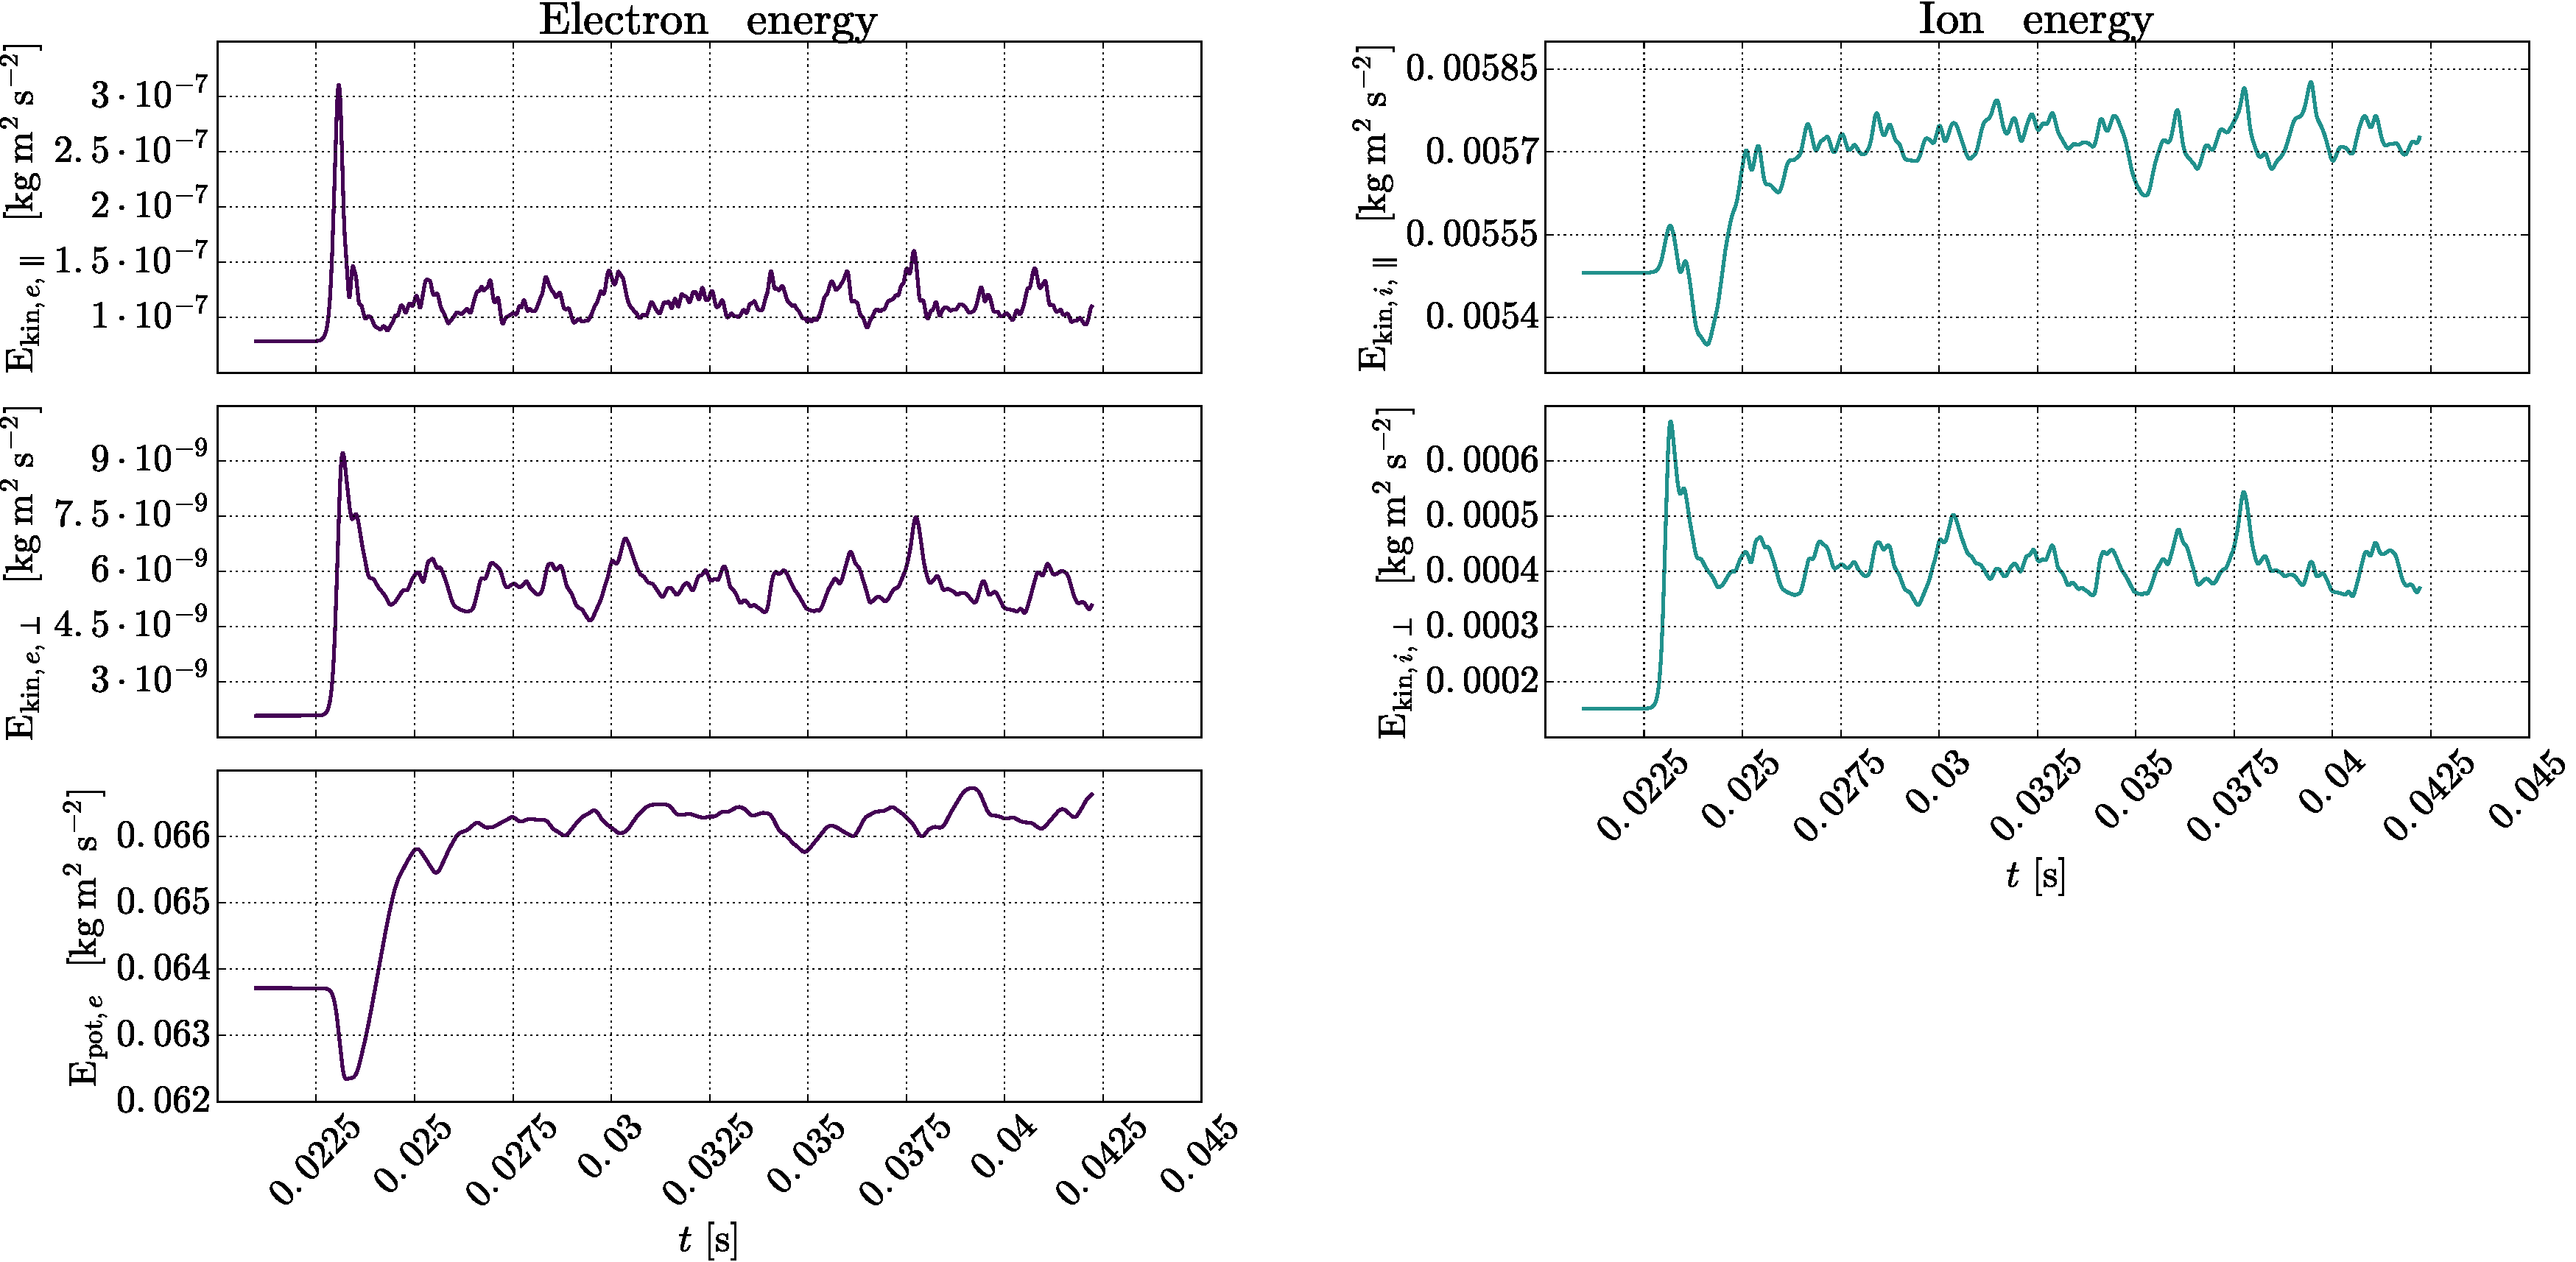
\includegraphics[width=1.0\textwidth]{fig/results/energyTrace/energyTraceB008}
    \caption{Time trace of the energy for $B=0.08$.}
    \label{fig:energyTrace008}
\end{figure}

As a consequence the eddies evolve at a faster phase, before the saturated turbulent state where eddies evolve at a slower rate, and the energy stays closer to the temporal mean (as seen in ...)
It is also important to observe that the fluctations can be big enough to push the plasma off center as observed in ...
%
\begin{figure}[htbp]
    \centering
    \begin{subfigure}[h]{1.00\textwidth}
        \centering
        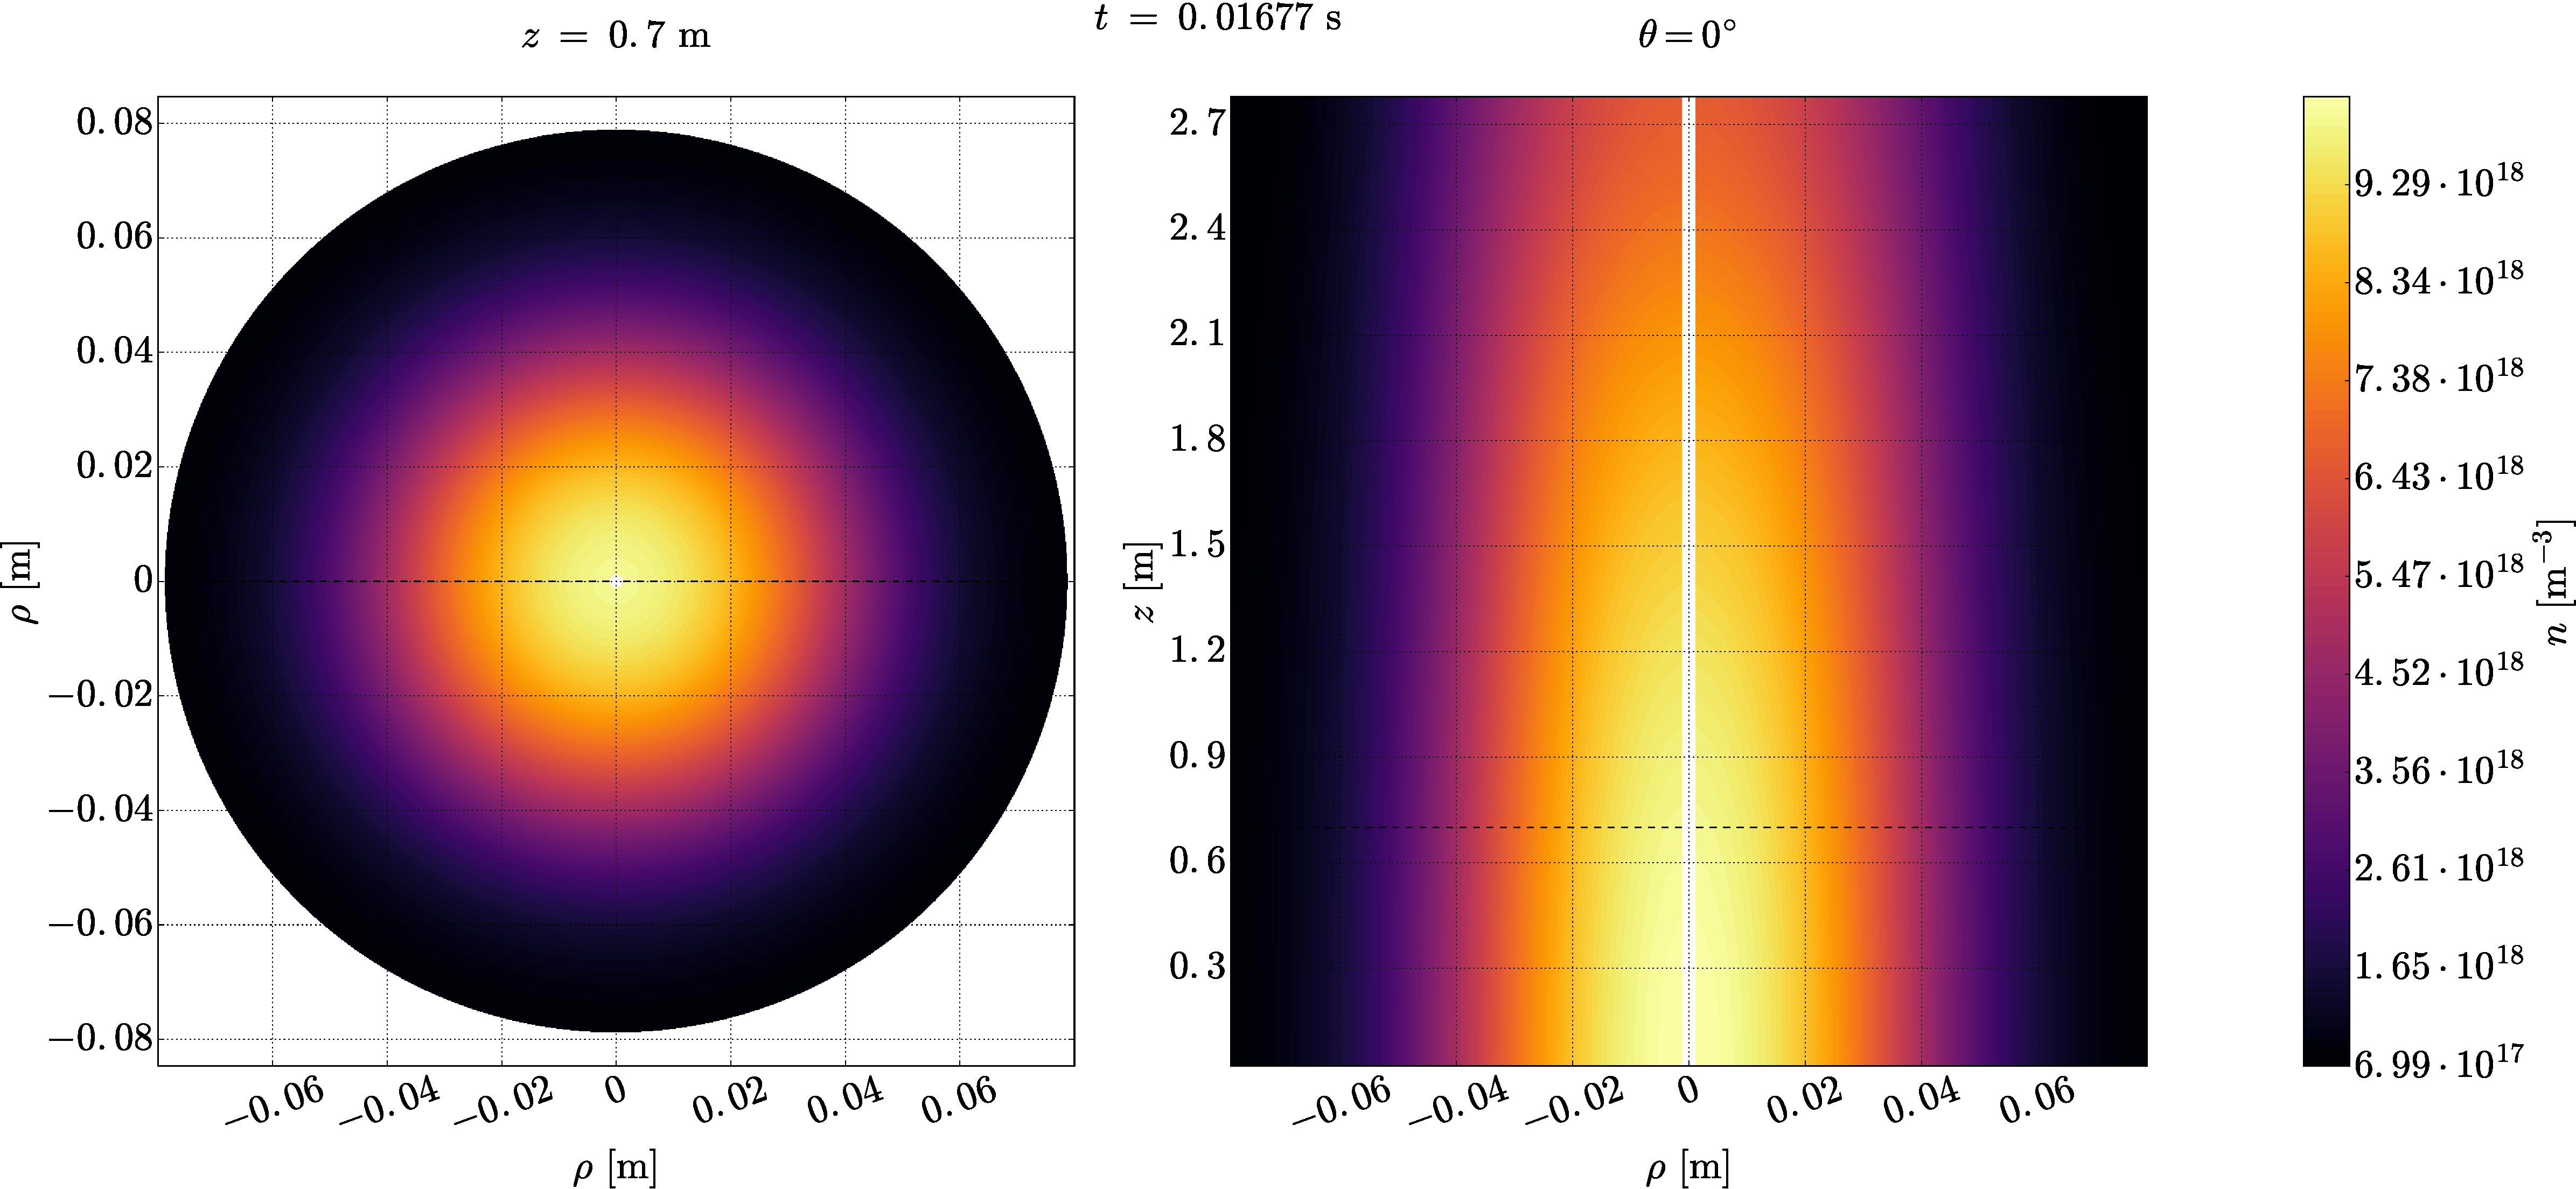
\includegraphics[width=1.0\textwidth]{fig/results/2DTurbulence/steadyStateN}
        \caption{The plasma at the steady state.}
        \label{fig:2Dsteady}
    \end{subfigure}%
    \\
    \begin{subfigure}[h]{1.00\textwidth}
        \centering
        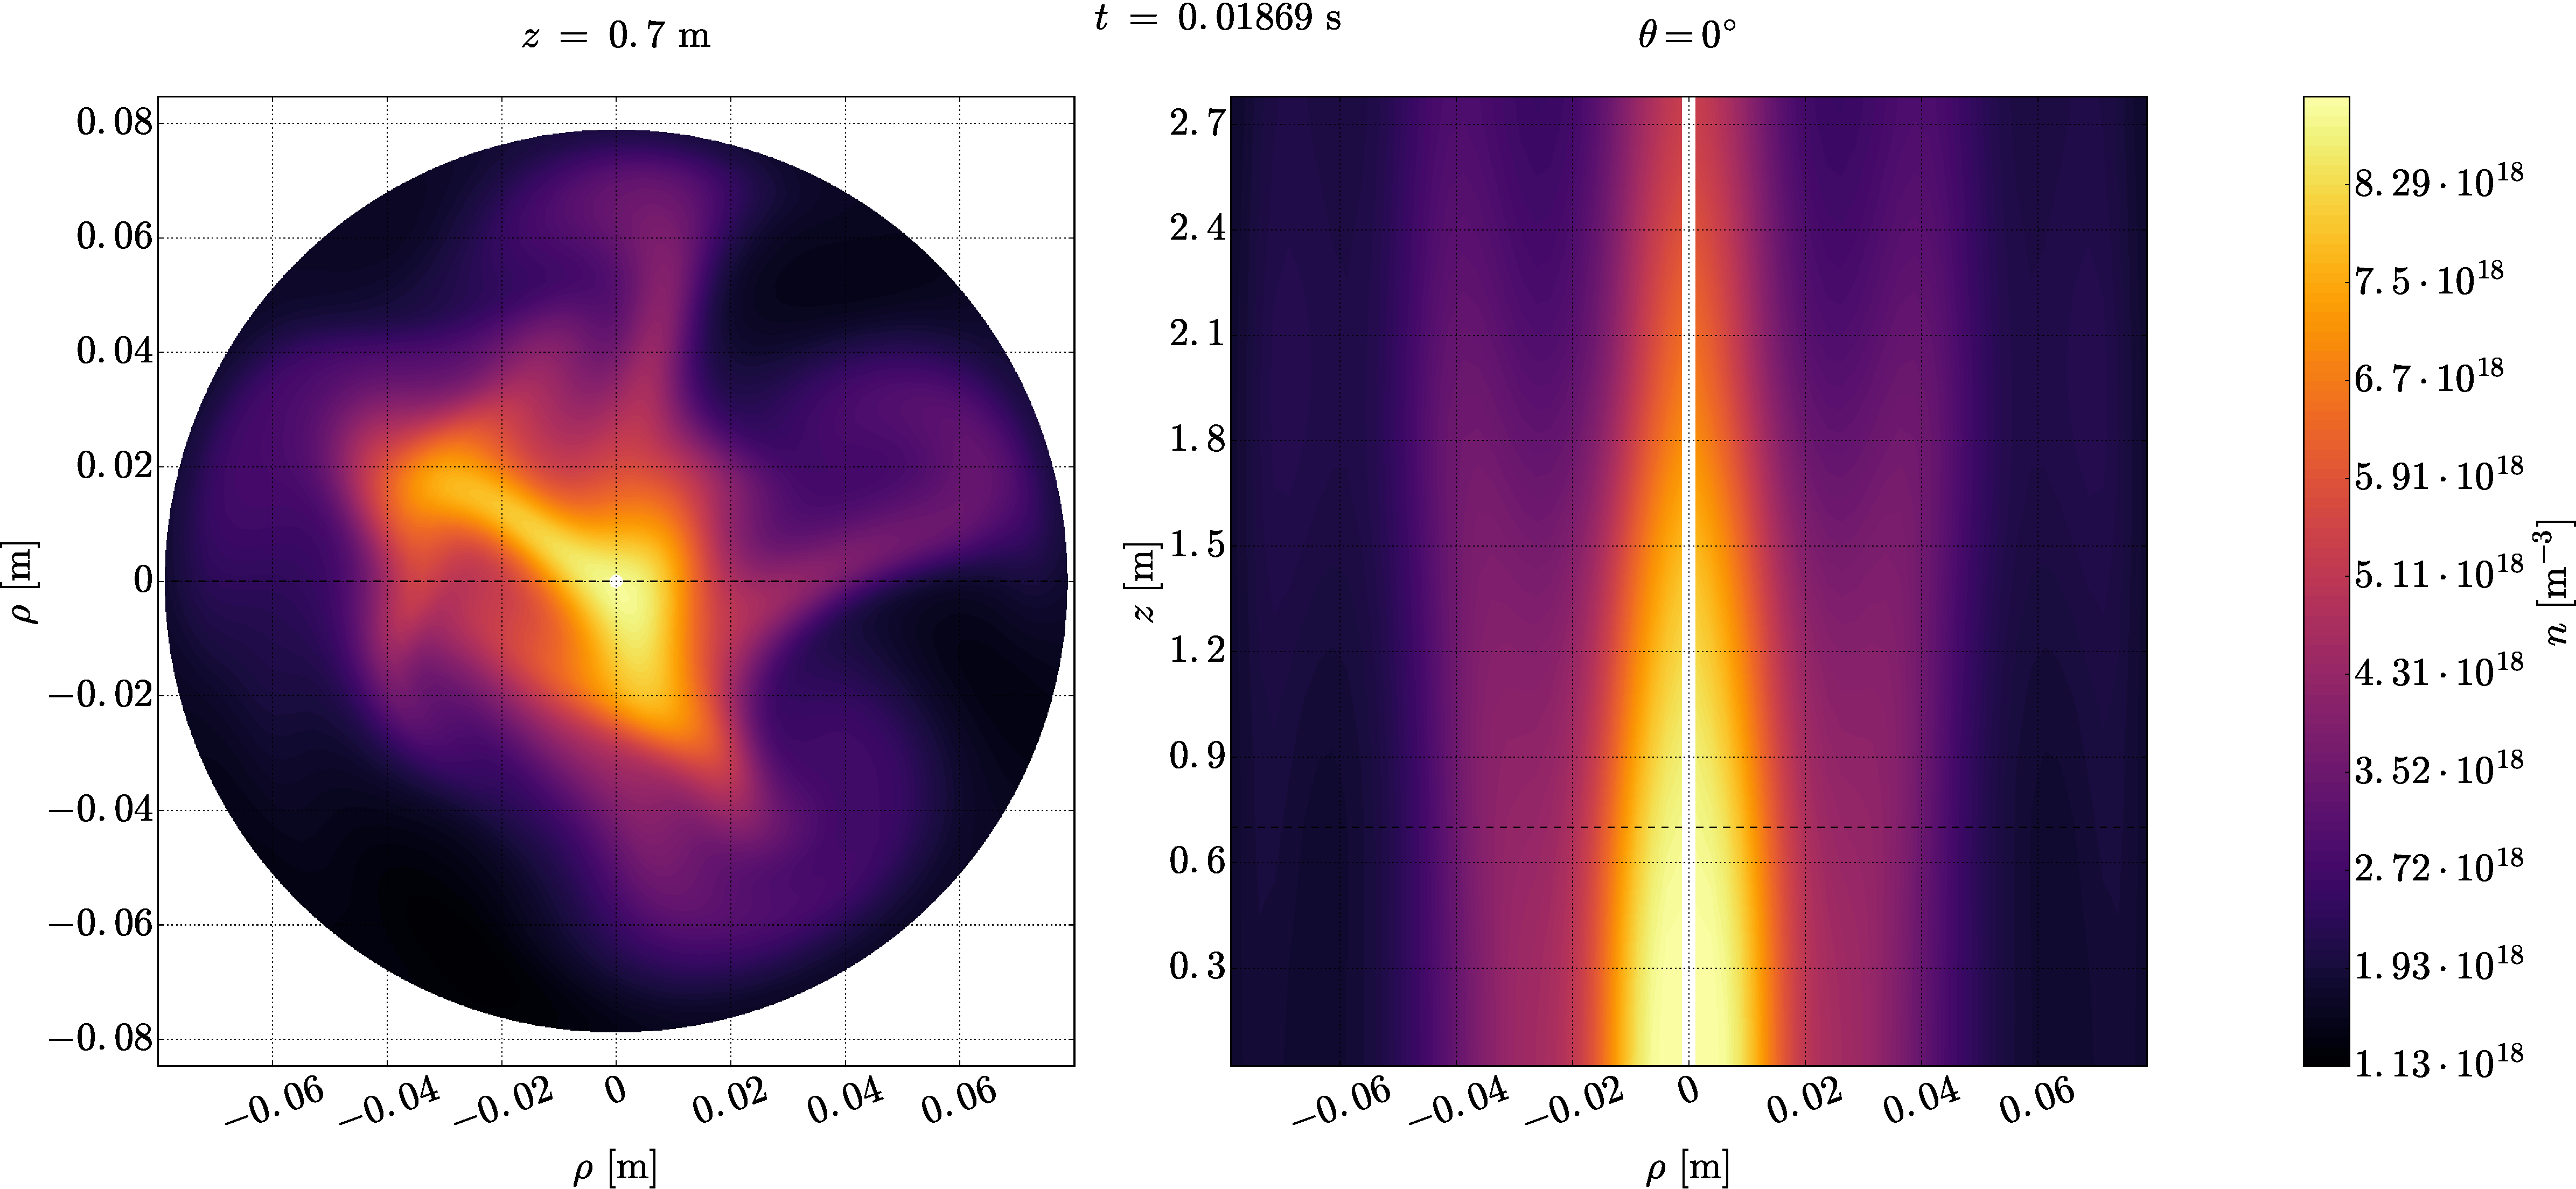
\includegraphics[width=1.0\textwidth]{fig/results/2DTurbulence/violentBurst}
        \caption{A violent burst is observed at the energy overshoot.}
        \label{fig:violentBurst}
    \end{subfigure}
    \\
    \begin{subfigure}[h]{1.00\textwidth}
        \centering
        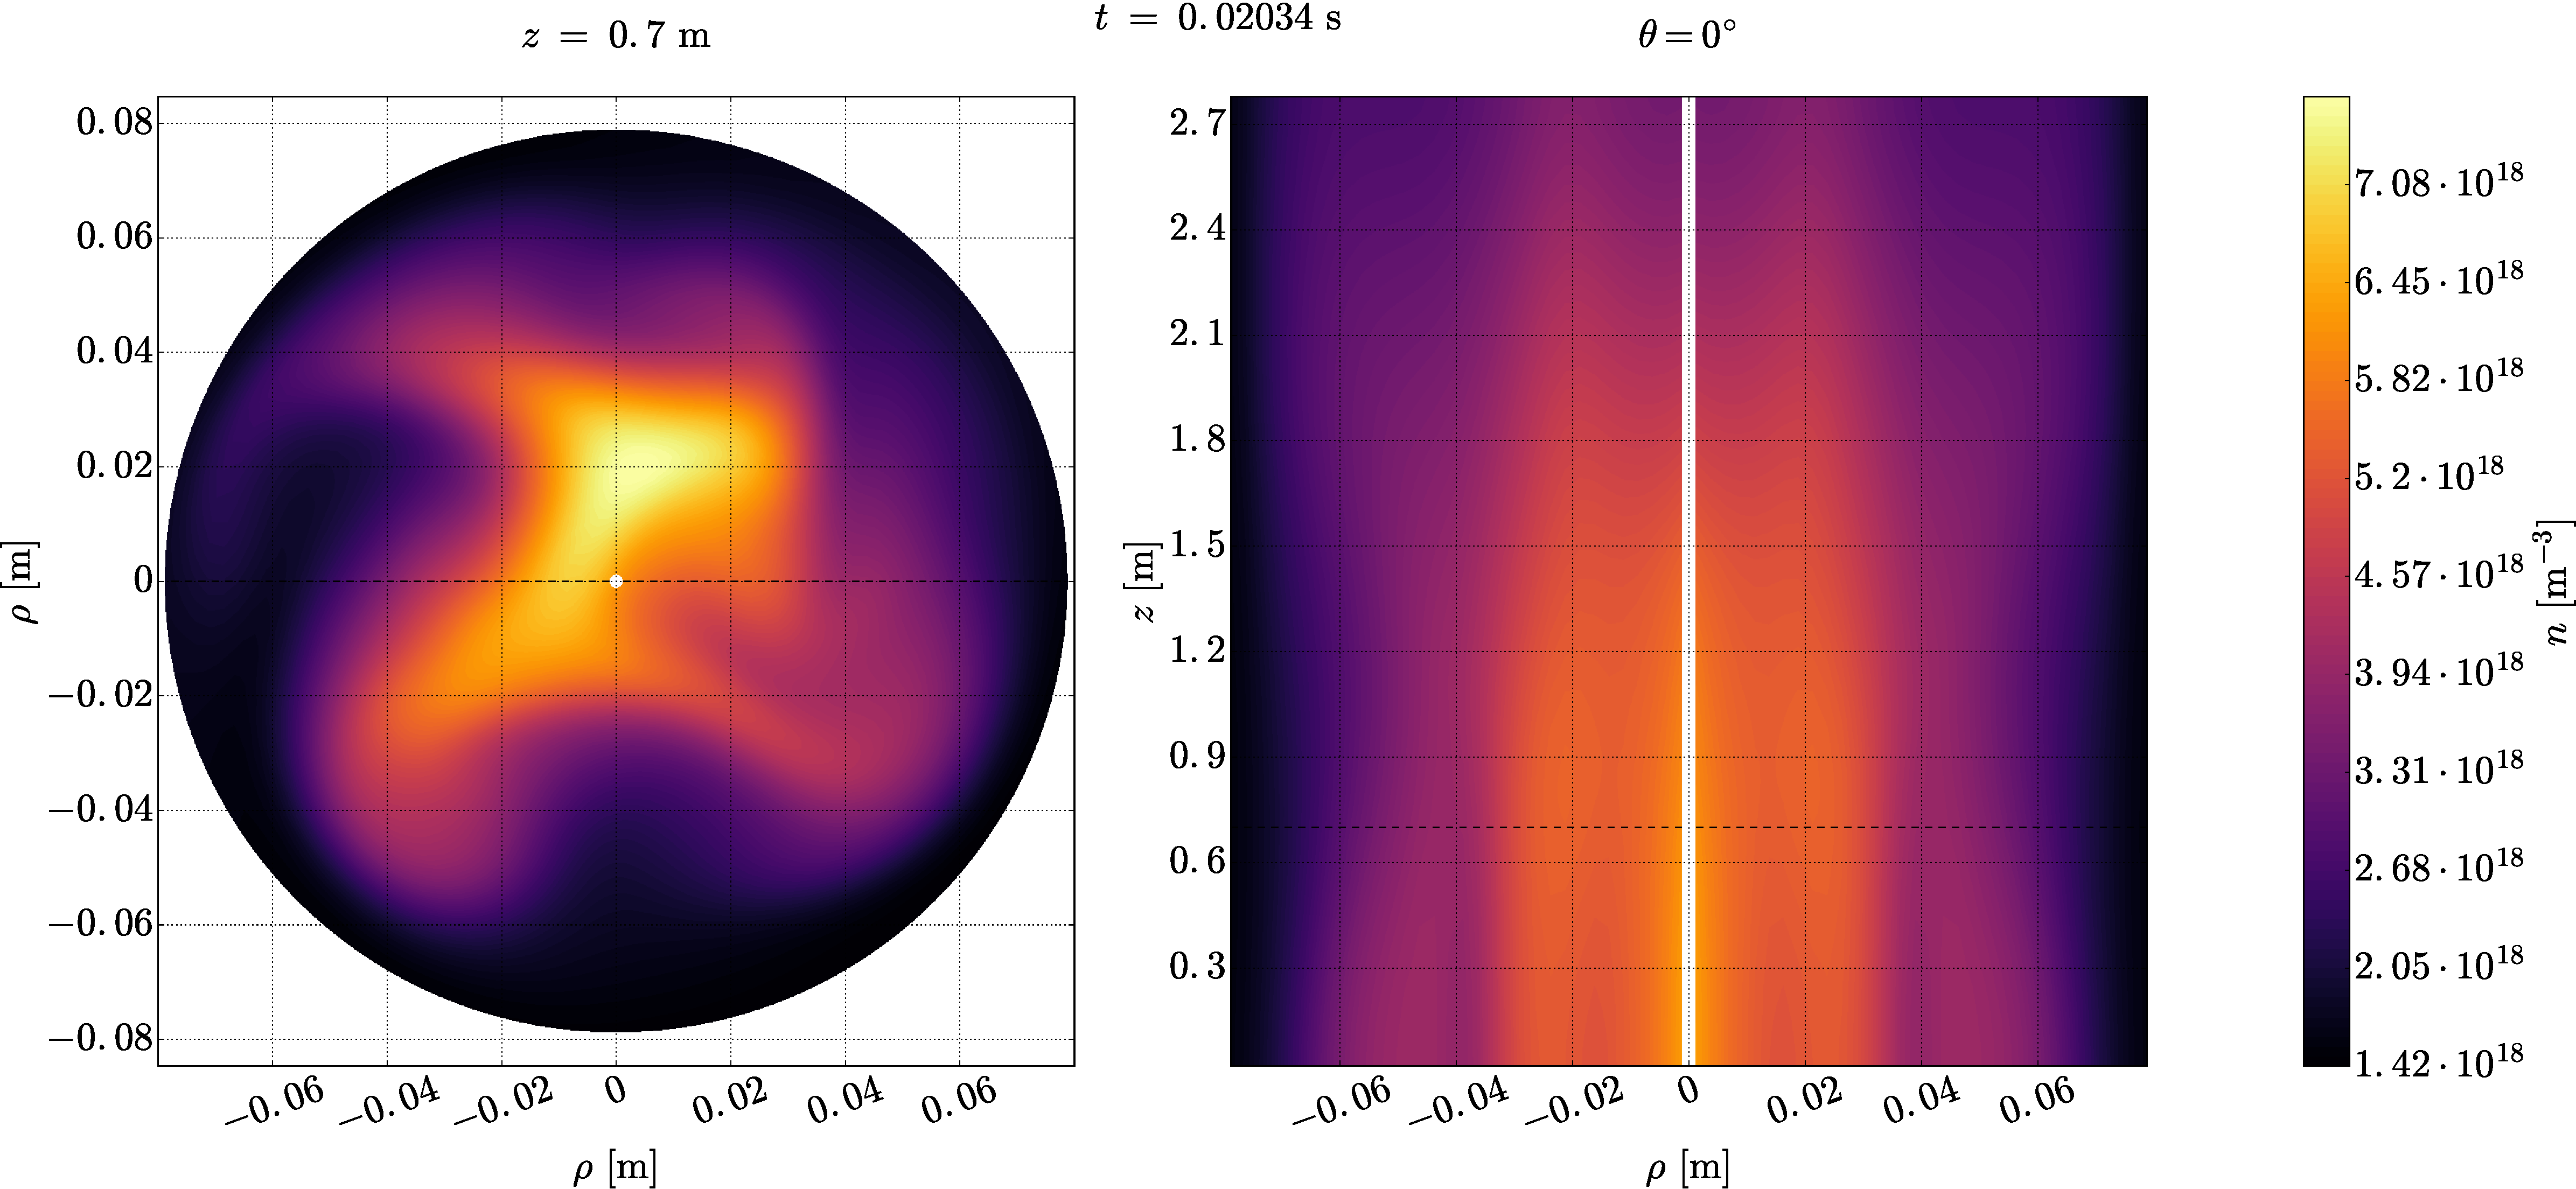
\includegraphics[width=1.0\textwidth]{fig/results/2DTurbulence/offCenter}
        \caption{Example of the plasma bulk being off axis}
        \label{fig:offcenter}
    \end{subfigure}
    \caption{Turbulent eddies are observed in the saturated turbulence state.
    Here shown for $B=0.1\T$}
\end{figure}
%
The fluctuations are no longer in an ordered pattern as they were in the linear phase, as shown in
%
\begin{figure}[htb]
    \centering
    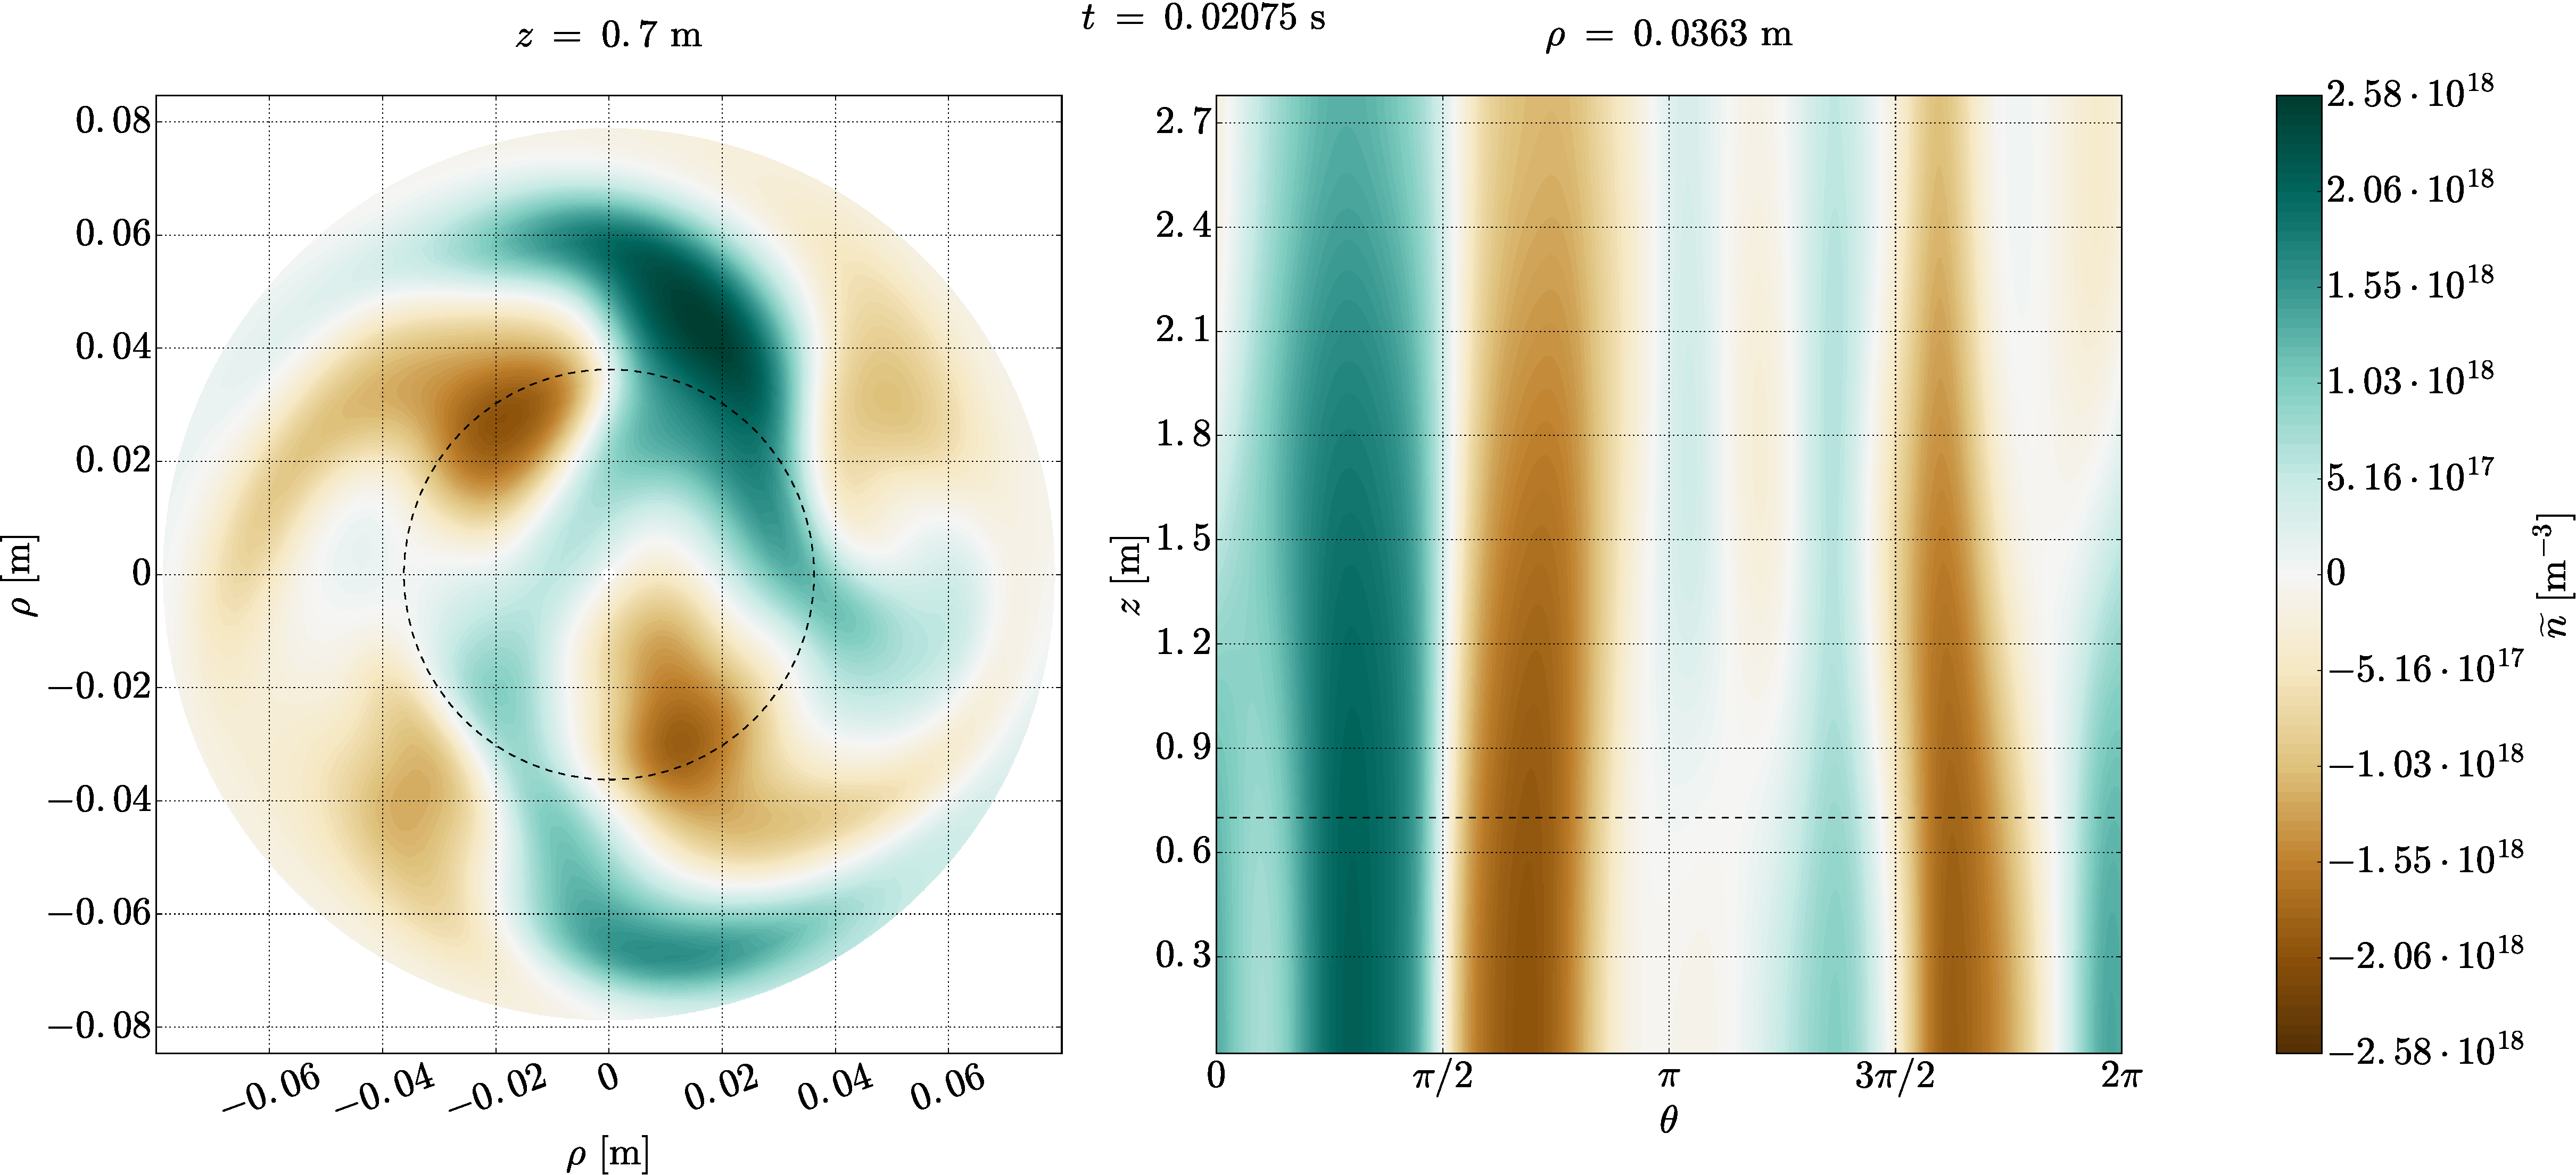
\includegraphics[width=1.0\textwidth]{fig/results/2DTurbulence/fluct}
    \caption{Fluctations in the turbulent state for $B=0.1\T$}
    \label{fig:2DFluct}
\end{figure}
%
